\documentclass[a4paper,10pt,notitlepage]{report}
\usepackage[utf8]{inputenc}
\usepackage{authblk}
\usepackage{geometry}
\usepackage{graphicx}
\usepackage{float}
\usepackage{cite}
\usepackage{caption}
\usepackage{subcaption}
\usepackage{hyperref}
\usepackage[numbers]{natbib}
\usepackage{rotating}
\usepackage{lineno}
\usepackage{amsmath}
\usepackage{amssymb}
\usepackage{enumitem}
\usepackage{cleveref}
\usepackage[titletoc]{appendix}

\makeatletter
\setlength{\@fptop}{0pt}
\makeatother

\pdfinfo{%
  /Title    ()
  /Author   (Lukasz Fulek)
}




%chapter heading
\makeatletter
\renewcommand{\@makechapterhead}[1]{%
 \vspace*{18\p@}%
  {\parindent \z@ \raggedright
%     \LARGE \bfseries \thechapter. #1\par\nobreak
%     \vskip 40\p@
      \Huge \bfseries \thechapter. #1\par\nobreak
      \vskip 40\p@
  }}
\makeatother


% Title Page
\title{\textbf{Measurement of particle production\\with Roman Pot detectors in diffractive proton-proton interactions at~$\sqrt{s}=$~200~GeV}\vspace*{10pt}}
\author[1]{Leszek Adamczyk}
\author[1]{Łukasz Fulek}
\author[2]{Włodek Guryn}
\author[3]{Bogdan Pawlik}
\author[1]{\mbox{Mariusz Przybycień}}
\author[1]{Rafał Sikora}
\affil[1]{AGH University of Science and Technology, FPACS, Kraków, Poland}
\affil[2]{Brookhaven National Laboratory, Upton, NY, USA}
\affil[3]{Institute of Nuclear Physics PAN, Kraków, Poland}

\setcounter{Maxaffil}{0}
\renewcommand\Affilfont{\itshape\small}
\renewcommand{\bibname}{References}

\begin{document}

\begin{center}
\begin{minipage}[c]{0.12\linewidth}%
\vspace{5.5pt}\textbf{\LARGE{of the}}
\end{minipage}
\begin{minipage}[c]{0.15\linewidth}%
\hspace*{-8pt}
\includegraphics[width=\linewidth]{graphics/STAR_logo.pdf}
\end{minipage}~
\begin{minipage}[c]{0.24\linewidth}%
\vspace{9pt}\hspace*{-8pt}\textbf{\LARGE{Experiment}}
\end{minipage}\\[-50pt]
\textbf{\LARGE{Analysis Note}}

\vspace*{110pt}
\begin{minipage}{\linewidth}
\maketitle
\begin{abstract}
	In this note we present the analysis of the diffractive measurement with the STAR Roman Pot detectors at~RHIC. The measurement is focused on the~spectra of identified charged particles as pions, kaons, protons and their antiparticle counterparts in Single Diffraction Dissociation $\left(p+p\to p+X\right)$ and Central Diffraction $\left(p+p\to p+X+p \right)$ processes. The~spectra of inclusive charged particles are also measured.
	Moreover, the~proton–antiproton production asymmetry as a~function of rapidity is presented and allows one  to study the~baryon number transfer over a~large space in rapidity in single diffraction. A~similar effect has been studied in proton-proton and proton-photon interactions but it is the first measurement in proton-Pomeron interaction. This data come from proton-proton collisions collected in 2015.
	The forward proton(s) were tagged in the STAR Roman Pot system while the charged particle tracks were reconstructed in the~STAR Time Projection Chamber (TPC). 
	Ionization energy loss of charged particles was used for particle identification. 
	We describe all stages of the analysis involving the extraction of efficiency and acceptance corrections, comparison of the data with MC simulations and systematic uncertainty studies.	
\end{abstract}
\thispagestyle{empty}
\end{minipage}

\vspace{100pt}

 \Huge{\textbf{\textit{DRAFT}}}
\end{center}


\clearpage
\thispagestyle{empty}
\newgeometry{hmargin={2cm, 2cm}, height=10.0in}
\tableofcontents



%% =====  DATASET ====
%%===========================================================%%
%%                                                           %%
%%                          INTRODUCTION                          %%
%%                                                           %%
%%===========================================================%%


\chapter{Introduction}\label{chap:introduction}

\section{Diffractive interactions in $pp$ collisions}
Diffractive processes at high energies are characterized by the exchange of the Pomeron, a color singlet object with quantum numbers of the vacuum described by the Regge theory \cite{barone}\cite{donnachie_dosch_landshoff_nachtmann_2002}. Due to non-perturbative nature of interactions, there are difficulties in applying QCD to diffraction. Experimentally, diffraction is identified as interaction with large rapidity gap, i.e. final states are separated in rapidity space.

There are two processes of interest, shown in Figure \ref{fig:sdcdgraph} (a, b), the Central $\left(\textnormal{CD: }p+p\to p+X+p\right)$ and Single $\left(\textnormal{SD: }p+p\to p+X\right)$ Diffractive scattering, where $X$ is the diffractive system. In CD interactions, two protons stay intact after the scattering, whereas in SD only one proton.
\begin{figure}[hb]
	\centering
	\parbox{0.484\textwidth}{
		\centering
		\begin{subfigure}[b]{\linewidth}{
				\subcaptionbox{\label{fig:cdgraph}}{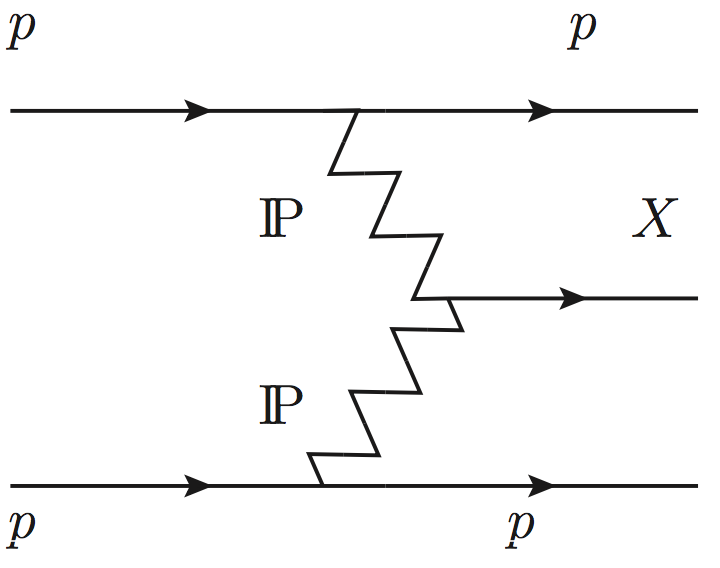
\includegraphics[width=\linewidth]{graphics/introduction/cd.png}}}
		\end{subfigure}
	}
	\quad
	\parbox{0.484\textwidth}{
		\centering
		\begin{subfigure}[b]{\linewidth}{
				\subcaptionbox{\label{fig:sdgraph}}{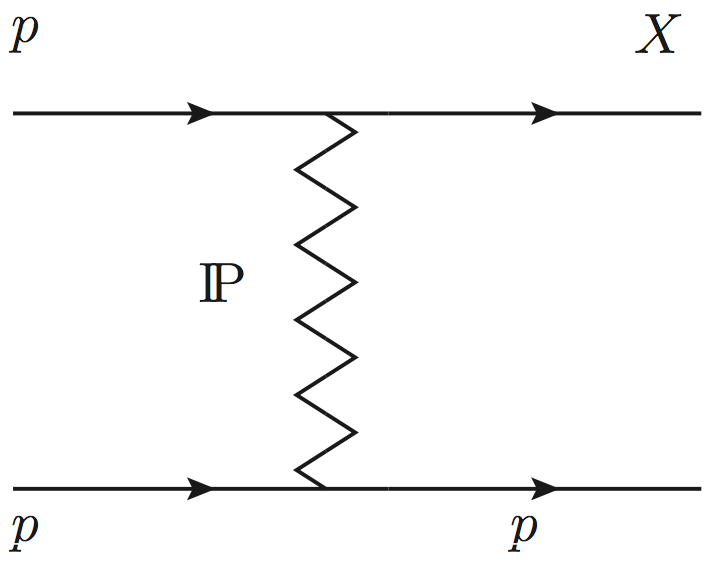
\includegraphics[width=\linewidth]{graphics/introduction/sd.png}}}
		\end{subfigure}
	}%
	\caption[Diagrams of Central Diffraction and Single Diffraction]{Diagrams of Central Diffraction (a) and Single Diffraction (b).}
	 \label{fig:sdcdgraph}
\end{figure}
The (identified) charged particle production in the mid-rapidity region has been widely studied in minimum bias inelastic hadron-hadron collisions starting from the very first experiments performed at ISR at CERN throughout contemporary measurements with very high center-of-mass energy at RHIC \cite{systmeasurhic} and LHC \cite{Adam:2015qaa}. This is the first measurement with tagged forward protons, 
which allows efficient identification of diffractive events. The measured particle spectra and ratios deliver information on collision dynamics, mechanism and allows to validate some phenomenological models and tune some general purpose MC generators.
\section{Baryon number transfer}
In the Standard Model the baryon 
number is conserved in all interactions. The conserved baryon number associated with the beam particles is called "baryon number transfer" and has been studied theoretically for some time~\cite{Kopeliovich:1988qm,Rossi:1977cy,Bopp:2000cr}. The baryon number transfer, which is quantified by the baryon to anti-baryon ratios, is often described as a function of the size of the transport in rapidity represented by
rapidy difference $\Delta y = y_{beam}-y$, where $y_{beam}=\ln\left(\sqrt{s}/m_p\right)$ is the rapidity of the beam and $y$ the rapidity of the particles produced in the central system. In~the~String Junction Model  \cite{Rossi:1977cy} the baryon number can be transferred over large distances in the rapidity. In this picture, baryon number transfer is exponentially suppressed as a function of the rapidity interval $\Delta y$. In particular, when there are only purely gluonic exchanges between the valence quarks of the proton, the baryon number transfer does not depend on the rapidity and approaches a constant and finite value~\cite{Kopeliovich:1988qm}. There is also a model \cite{Bopp:2000cr}, in which the initial baryon may end up at the backward end of the diffractive system. The~edge of the rapidity gap $\Delta\eta$ is related to the~relative proton momentum loss $\xi=\Delta E/E$, $\Delta\eta\approx-\ln\xi=-\ln\left(M_X^2/s\right)$. %Therefore, the measurement of particle ratios as a function of $\xi$ of the outgoing protons should be taken into account to validate this model. 
There is a large number of the experimental data available on baryon number transfer \cite{Aamodt:2010dx}. The mid-rapidity  anti-proton to proton ratio is sensitive to center-of-mass energy  and varies between $0.4$ for ISR energies and almost $1$ for the~LHC, where the~transfer size in the rapidity space $\Delta y$ is large and equals to almost $9$ units. In addition, this effect was also measured by the H1 Collaboration in proton-photon interactions \cite{Kopeliovich:1998ps}, where the data show that there is a sizeable baryon to anti-baryon asymmetry. The similar effect can be studied in SD interactions, where the direction of the initial baryon is uniquely defined.

%---------------------------

%---------------------------

%%%===========================================================%%
%%                                                           %%
%%                          EXPERIMENTAL SETUP                          %%
%%                                                           %%
%%===========================================================%%


\chapter{Experimental setup}\label{chap:experimentalsetup}
Measurement of diffractive events requires many subdetectors of the STAR experiment \cite{Ackermann:2002ad}, whose scheme is drawn in the Figure \ref{fig:starscheme}.
The main part of the~STAR detector is the TPC, the tracking detector, which provides information about momentum  and ionization energy loss $dE/dx$ of charged particles with $p_T \geq 100$~MeV/c in the full azimuthal coverage $\left(0\leq \phi \leq 2\pi\right)$ and a~pseudorapidity coverage of $-1.2 \lesssim \eta \lesssim 1.2$. The particle identification (PID) capability of the STAR experiment was improved by the Time-Of-Flight (TOF) system \cite{Llope:2009zz},  which measures TOF with resolution of about $100$~ps. 
\begin{figure}[hb]
	\centering
	
	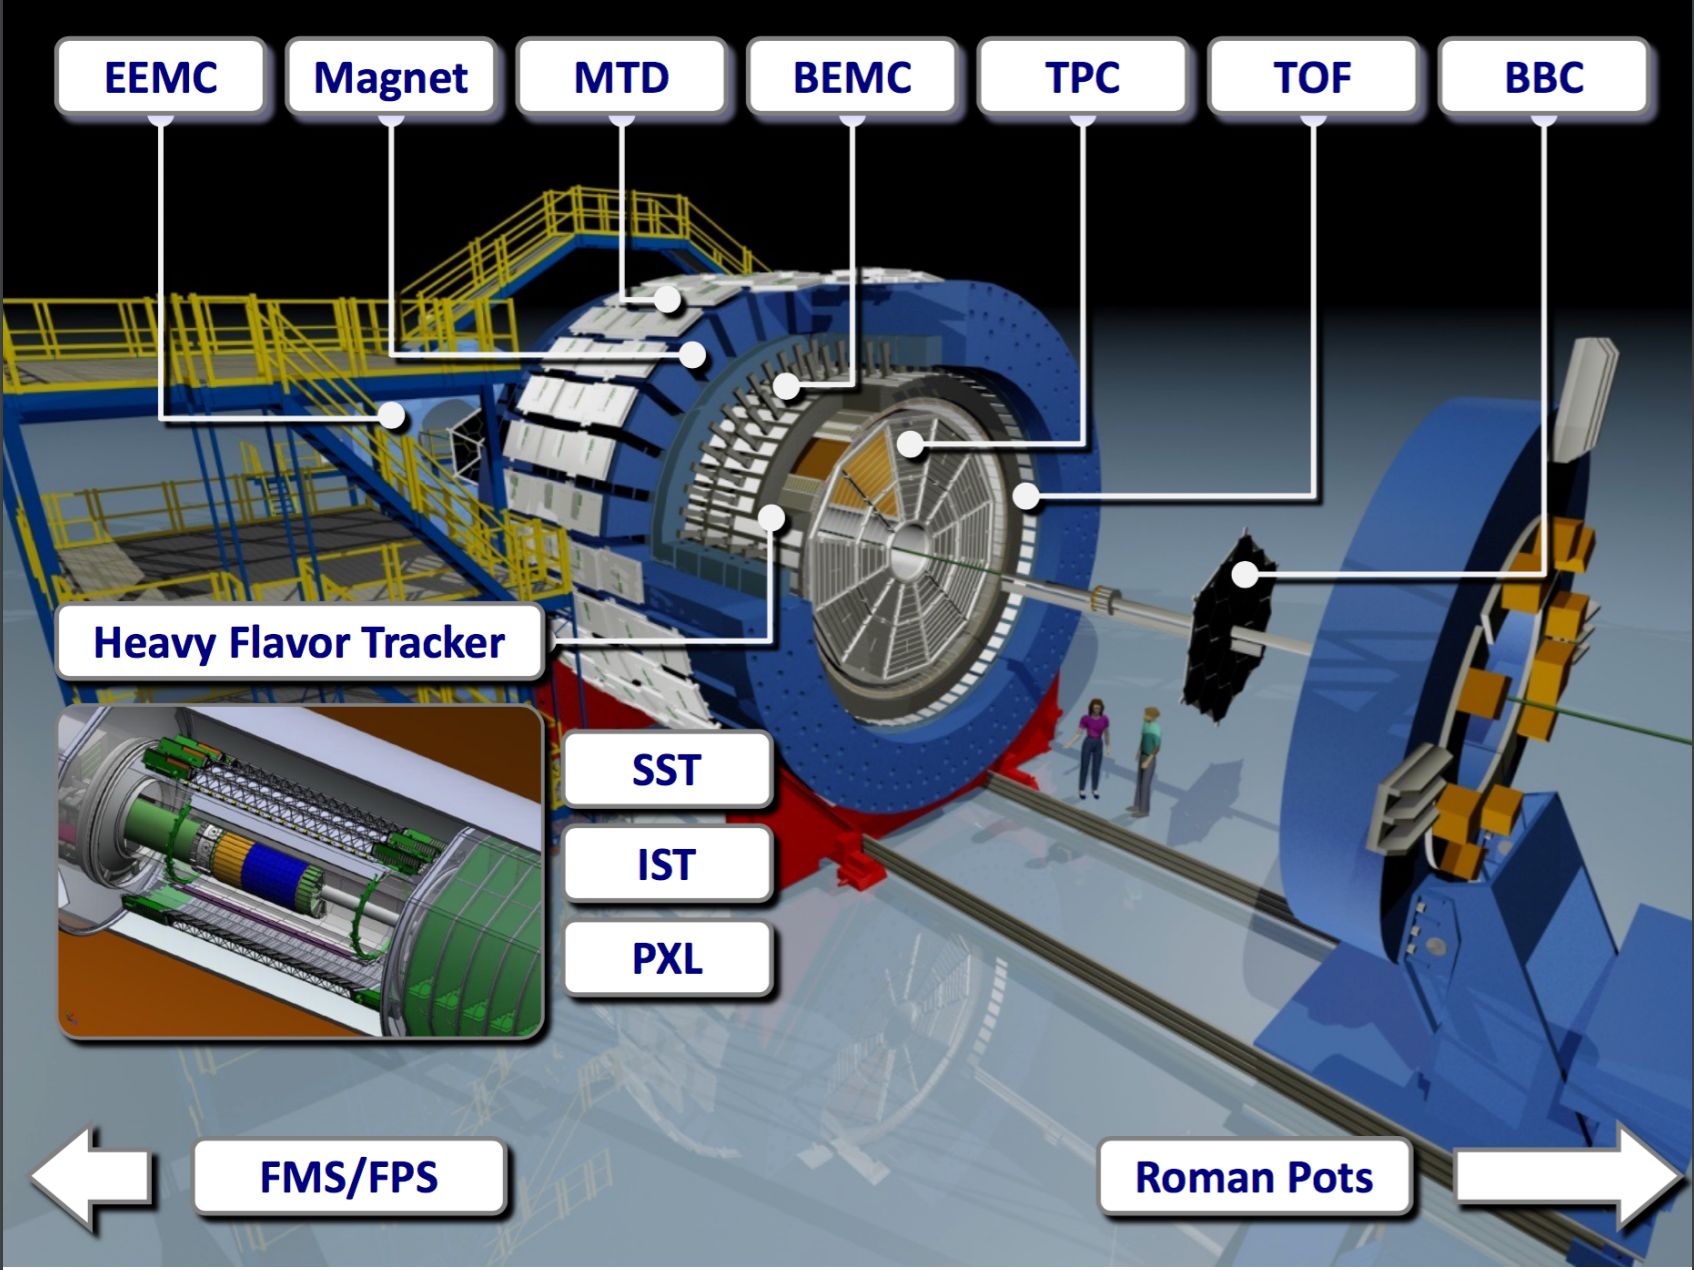
\includegraphics[width=0.9\linewidth]{graphics/experimentalSetup/star.png}
	
	\caption[Perspective view of the STAR detector, with a cutaway for viewing inner detector systems as configured in 2015.]{ Perspective view of the STAR detector, with a cutaway for viewing inner detector systems as configured in 2015.}
	\label{fig:starscheme}
\end{figure}

System of forward detectors in STAR \cite{A_N}, whose scheme is drawn in the Figure \ref{fig:rpscheme}, consists of  four stations of the Roman Pots (RP), two of each placed symmetrically with respect to the Interaction Point (IP), with two Silicon Strip Detector (SSD) packages in each station. The stations are located between RHIC DX and D0 dipole magnets at distances $15.8$ and $17.6$~m from  the IP. Each SSD package, housed inside the RP vessel, consists of four silicon planes and the~scintillator counters used for triggering. The acceptance of the RPs limits the kinematics of the protons to the~values of squared four-momentum transfer (Mandelstam $t$), $0.03\leq -t \leq 0.3$~GeV$^2/$c$^{2}$, and fractional momentum loss of the proton $\xi<0.6$.

\begin{figure}[hb]
	\centering
	
	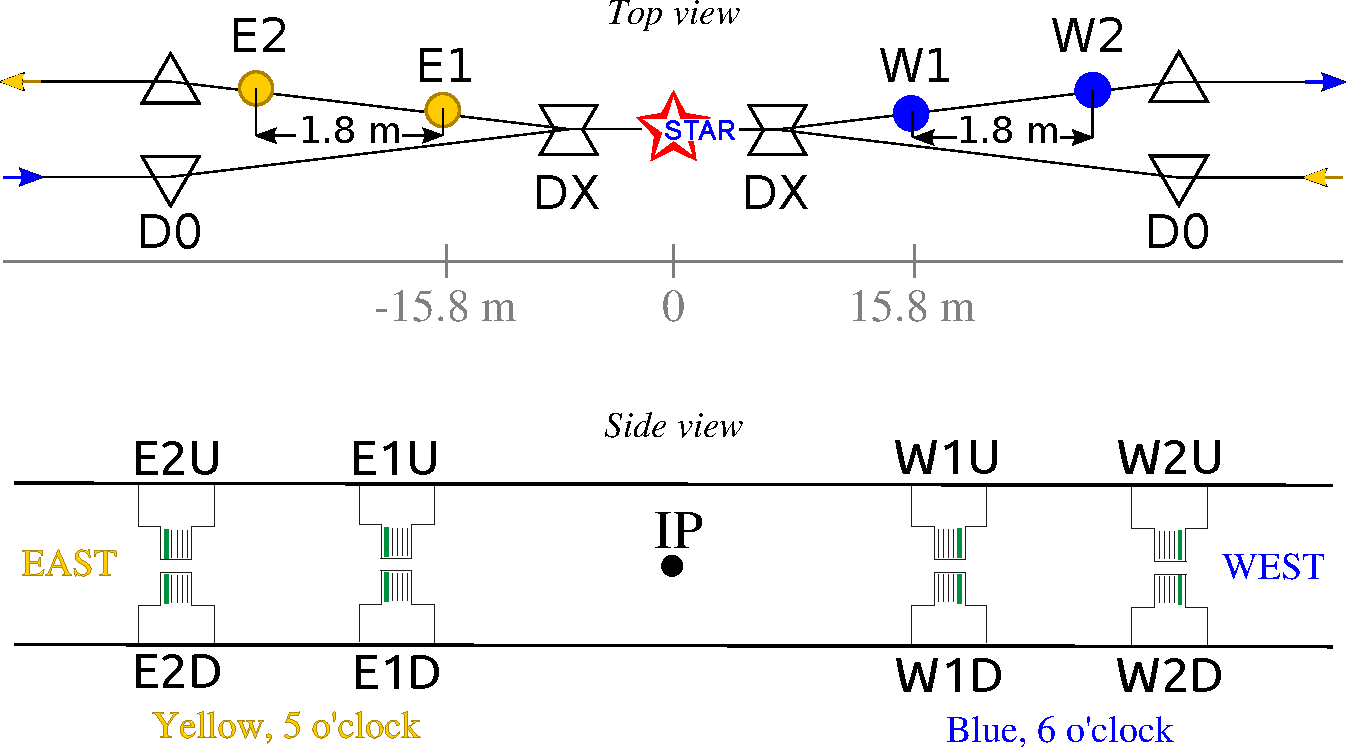
\includegraphics[width=\linewidth, page=1]{graphics/experimentalSetup/RP_phaseII_2.pdf}
	
	\caption[Layout of the Roman Pot system in STAR.]{ Layout of the Roman Pot system in STAR. The RPs are located between RHIC DX and D0 magnets  at distances $15.8$ and $17.6$~m. In each station two SSD packages, each consisting of four silicon planes and scintillator counters, are housed inside the RP vessels.}
	\label{fig:rpscheme}
\end{figure}

The trigger selection of diffractive events includes: tagging forward 
proton in the RP,  and Beam-Beam Counter~\cite{Kiryluk:2003aw} (BBC) and Zero Degree 
Calorimeter \cite{Adler:2000bd} (ZDC) veto on the outgoing proton side. Additionally, BBC is used as a tagger of diffractive state $X$ in SD events. The ZDCs are located at $18$~m from the IP and their purpose is to detect the neutral particles emitted within small solid angle. BBCs are scintillator-based detectors, used for the~luminosity measurement.
%\section{Bad runs}
% \subsection{SSD detecting efficiency}
% \subsection{Reconstruction efficiency}
%\label{sec:badRuns}

%---------------------------

%---------------------------

\section{Reconstruction}\label{sec:reconstruction}
Raw data was processed with the library version SL17f with the following BFC options:
\vspace{1em}

\noindent\texttt{DbV20160418,pp2015c,btof,mtd,mtdCalib,pp2pp,-beamline,beamline3D, \newline UseBTOFmatchOnly,VFStoreX, fmsDat,fmsPoint,fpsDat,BEmcChkStat,-evout,  \newline CorrX,OSpaceZ2,OGridLeak3D,-hitfilt}
\vspace{1em}

The \texttt{UseBTOFmatchOnly} option was used to form the vertices only from the global TPC tracks matched with TOF hits. It was found that this option provides better signal reconstruction efficiency and resolutions. 

The produced MuDst files (standard STAR data format) were further reduced to Cracow's picoDst data format. 

\chapter{Analysis}\label{chap:analysis}
\section{Event selection}
\subsection{SD and CD}
\begin{enumerate}
	\item Exactly one primary vertex with TPC tracks matched with hits in TOF.
	\item The reconstructed vertex is required to be within $80$~cm of the detector center along the  beam direction.
	\item At least two primary TPC tracks $N^{primary}_{reco}$ matched with hits in TOF and satisfying the selection criteria described in  \ref{chap:trackCut}.
	\item If there are exactly two primary tracks satisfying the above criteria and exactly two global tracks used for vertexing (Table \ref{tab:trackCutVertex}), the longitudinal distance between these tracks $|\Delta z_0|<2$~cm.
\end{enumerate}
\subsection{SD}
\begin{enumerate}
	\item SDT trigger 
	\item RP trigger on only one side of the STAR central detector (veto EAST \&\& WEST)
	\item RP trigger on only UP or DOWN  stations (veto UP \&\& DOWN)
	\item Any signal in small BBC tiles or ZDC on the opposite side of the STAR central detector to the triggered RP station(s).
	\item RP trigger on exactly two RP stations.
	\item Exactly one RP global track in the above RP stations with proton fractional momentum loss $0.02 < \xi < 0.4$.
\end{enumerate}

\subsection{CD}
\begin{enumerate}
	\item CPT2 trigger 
	\item Exactly one RP global track on each side of the STAR central detector with proton fractional momentum loss $0.02 < \xi_1,\xi_2 < 0.4$.
\end{enumerate}
\section{Track selection}\label{chap:trackCut}
For this analysis several track quality cuts are applied as shown in Table \ref{tab:trackCut}. Tracks are required to have at least $25$ fit points, ratio of fit points to possible fit points $N_{fit}/N_{poss}>0.52$, $15$ $dE/dx$ points, transverse impact parameter $d_0<1.5$~cm, and have a $\textrm{DCA}_{xy}<1.5$~cm, $\textrm{DCA}_{z}<1$~cm. Tracks are accepted within a pseudorapidity window of $-0.7$ to $0.7$.
The cuts listed in the Table \ref{tab:trackCut} on the number of Fit Points and ratio of Fit Points over Possible Fit Points are standard cuts used to reject low quality TPC tracks and avoid track splitting effects. The global
$\textrm{DCA}$ cut is used to select tracks that originate from the primary interaction vertex. The cut
on $dE/dx$ points is used to ensure that selected tracks have sufficient energy loss information
for particle identification purposes. Singly charged particles
must have a minimum $p_T$ of $0.15$~GeV/c to exit the TPC
in the $0.5$ Tesla magnetic field. In this analysis tracks
are required to have $p_T > 0.2$~GeV/c. For the identified
particle results in this paper, the pseudorapidity region is restricted
within $|\eta| < 0.7$ (i.e. mid-rapidity). The full $2\pi$ azimuthal coverage of the TPC is utilized.

	\begin{table}[H]
		\centering
		\begin{tabular}{| l | l |}
			\hline			
			Quantity & Cut \\
			\hline
			\hline
			Number of Fit Points & Fit Points $>24$\\
			Transverse Impact Parameter & $|d_0|<1.5$~cm\\ 
			Global Track Distance of Closest Approach to the primary vertex & $\textrm{DCA}_{xy}<1.5$~cm, $|\textrm{DCA}_{z}|<1.$~cm\\
			Ratio of Fit Points / Possible Fit Points & Fit Points/ Possible Fit Points $>0.52$\\
			$dE/dx$ Fit Points & $dE/dx$ Fit Points $>14$\\
			Primary Track Transverse Momentum & $p_{T}>0.2$~GeV/c\\
			Pseudorapidity & $|\eta|<0.7$\\
			TOF Matched Track & TOF Match-Flag $\geq1$\\
			\hline  
		\end{tabular}
		\caption[Analysis Track Level Cuts]{Analysis Track Level Cuts}
		\label{tab:trackCut}
	\end{table}
	
\begin{figure}[H]
	\centering
	\parbox{0.484\textwidth}{
		\centering
		\begin{subfigure}[b]{\linewidth}{
				{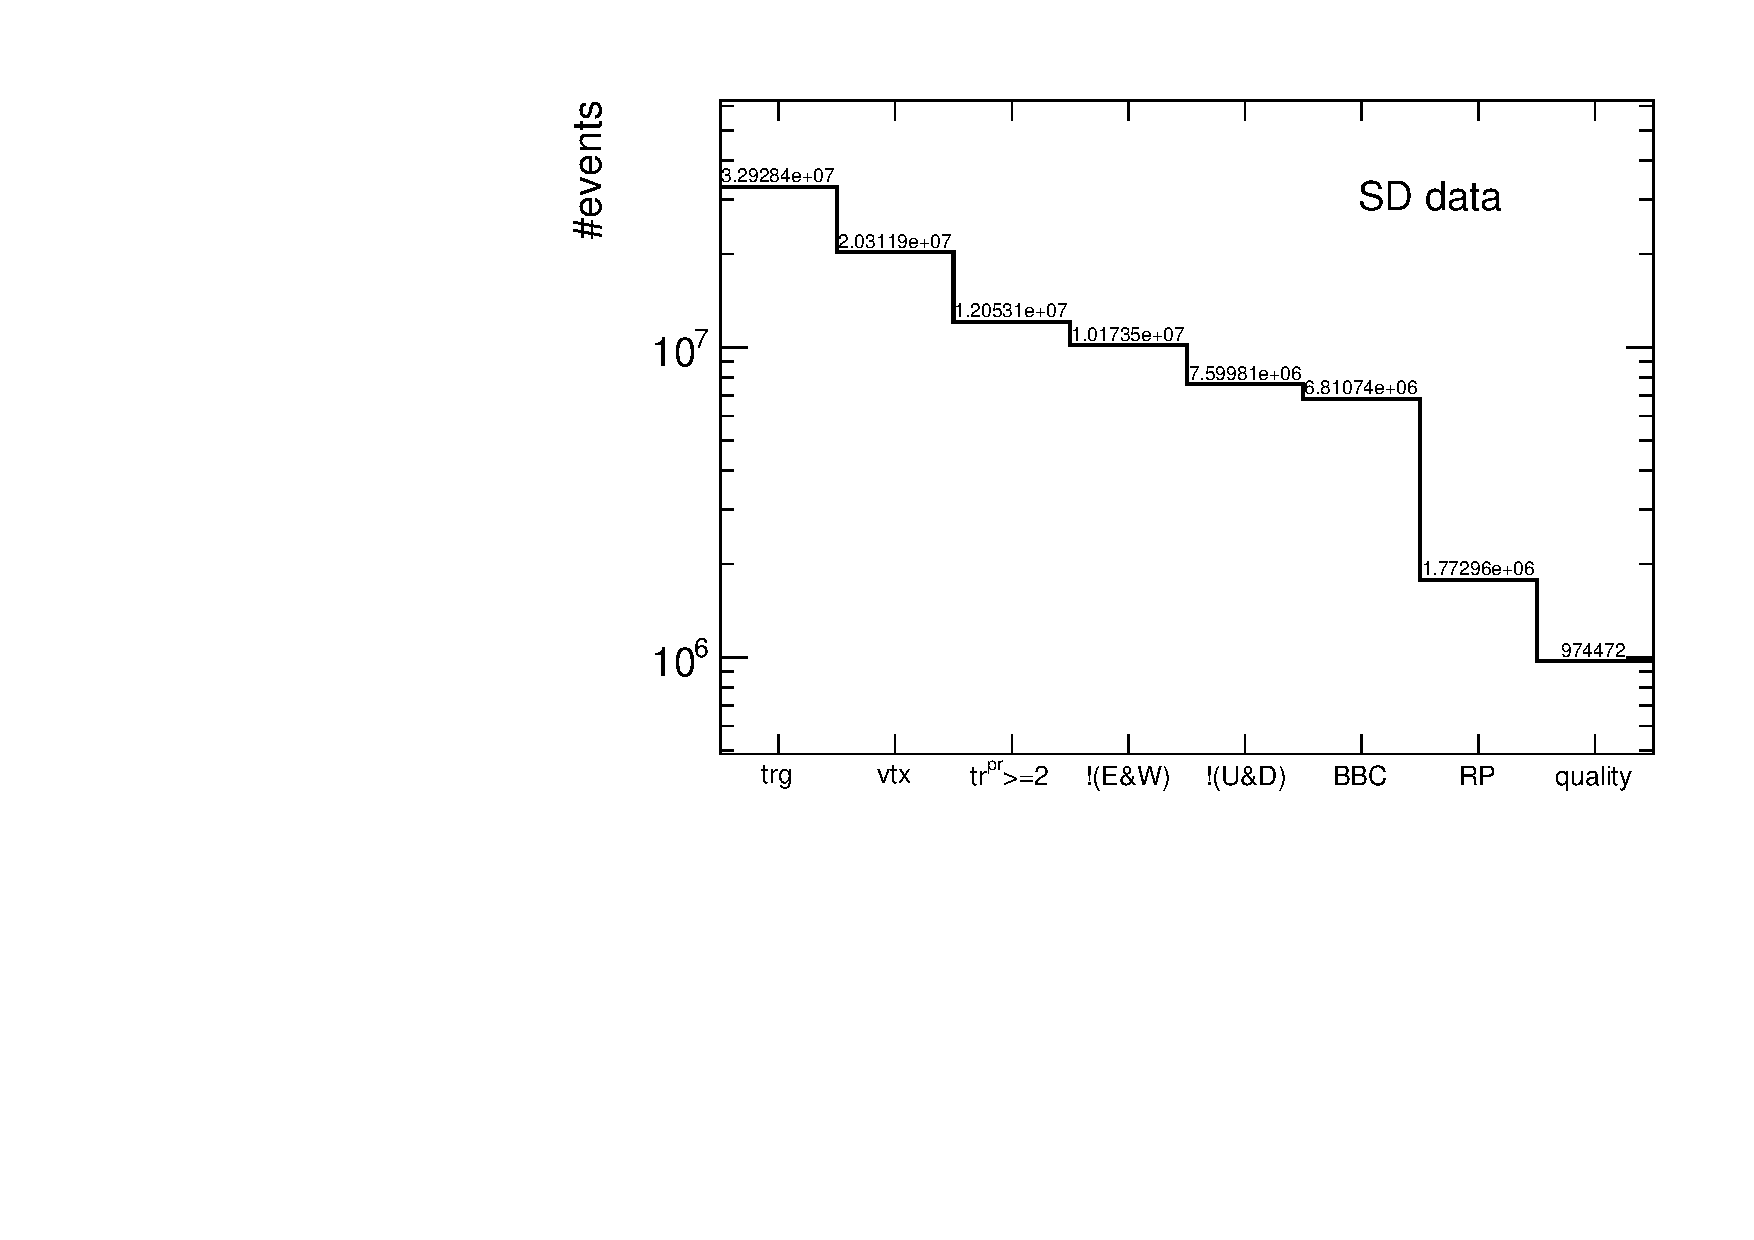
\includegraphics[width=1.04\linewidth, page=1]{graphics/cutFlow/SDT.pdf}}}
		\end{subfigure}
	}
	\quad
	\parbox{0.484\textwidth}{
		\centering
		\begin{subfigure}[b]{\linewidth}{
				{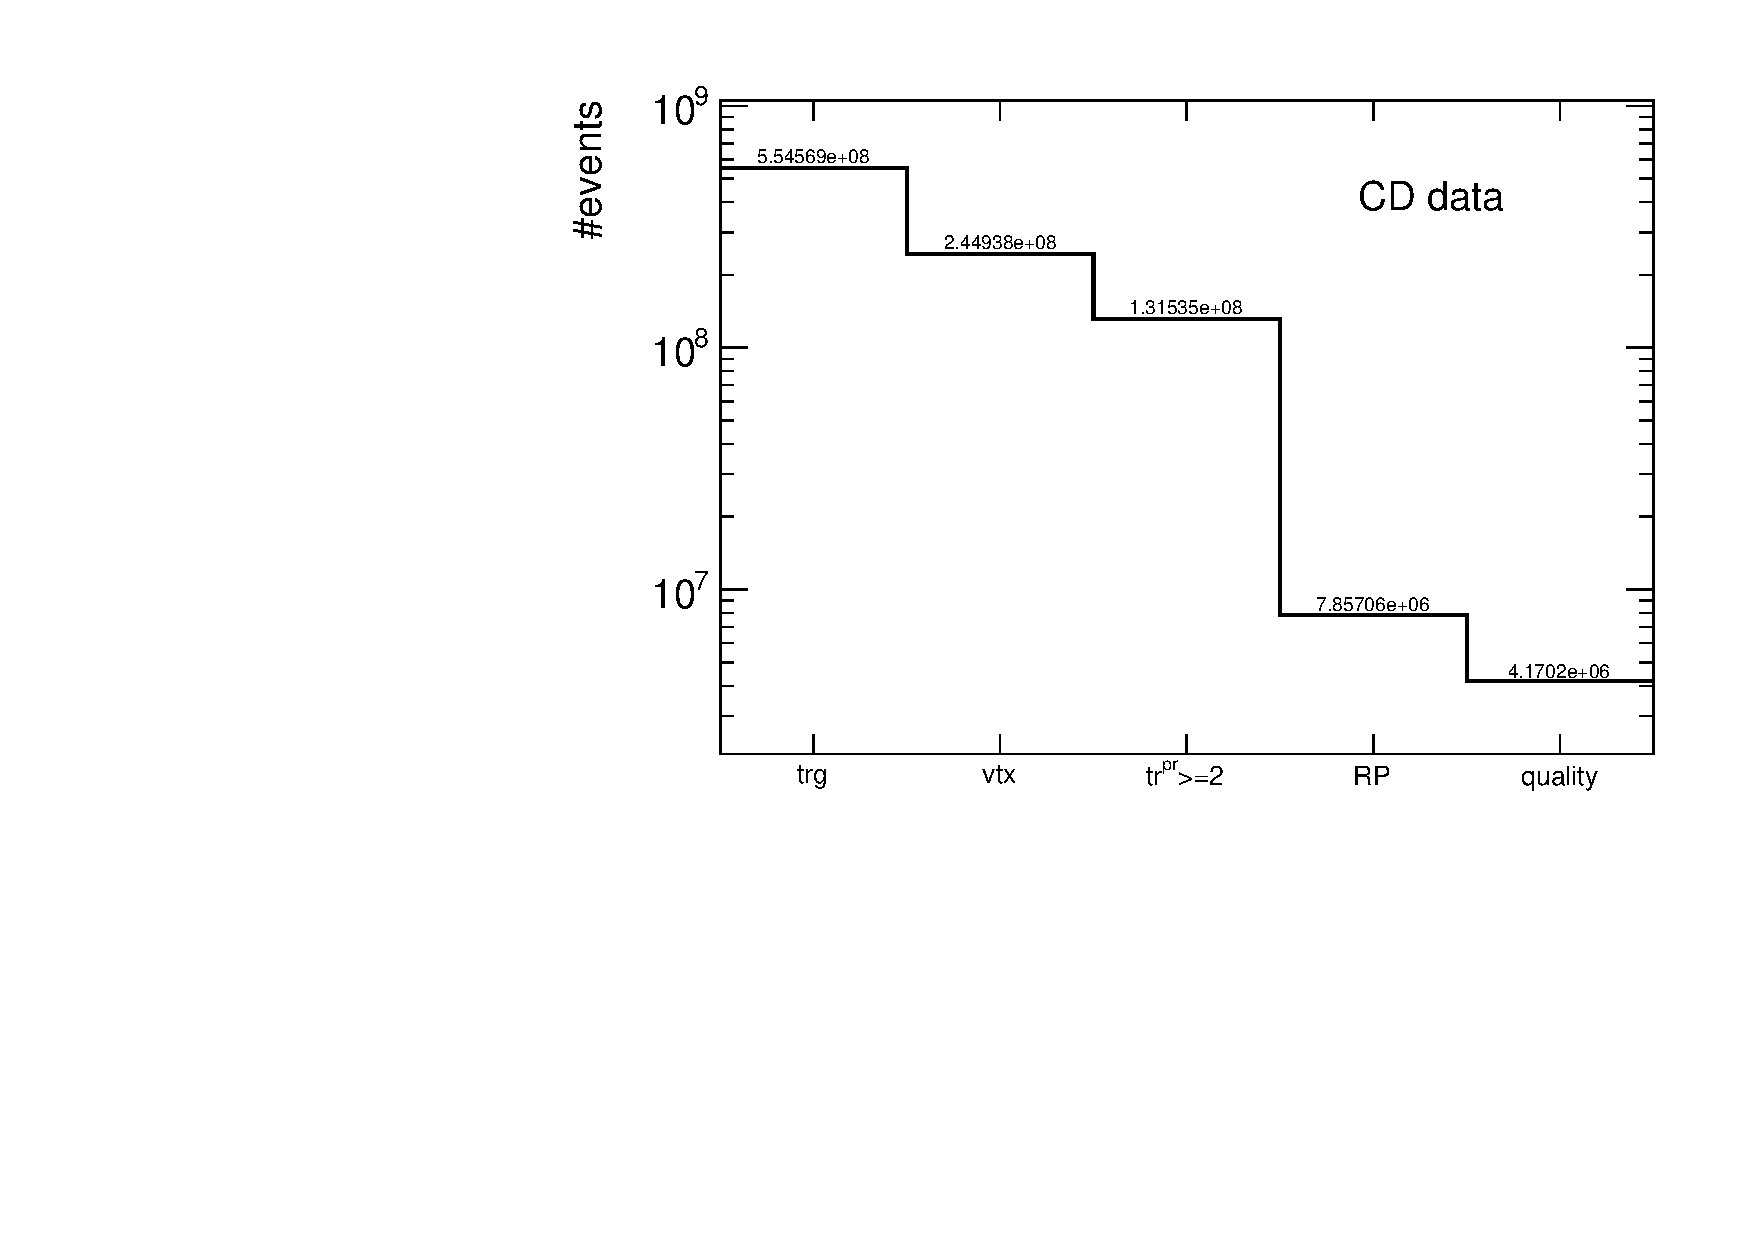
\includegraphics[width=1.04\linewidth, page=1]{graphics/cutFlow/CPT2.pdf}}}
		\end{subfigure}
	}
	\caption[Number of accepted events  after applying each event selection cut]{Number of accepted events  after applying each event selection cut. }
	\label{fig:selectionCutFlow}
\end{figure}


\section{Accidental background study}

The accidental backgrounds (same bunch pile-up background) are quantified using data-driven method. This includes any single(double)-side proton signal collected in coincidence with a diffractive like signal in the TPC-TOF detector. This type of background may come from the overlap of:
\begin{enumerate}
	\item RP:
	\begin{itemize}
		\item proton from beamhalo,
		\item low mass SD process without activity in TOF,
		\item elastic or low mass CD processes with undetected proton on the other side,
	\end{itemize}
	\item TPC+TOF:
	\begin{itemize}
		\item any central activity (dominantly from ND events).
	\end{itemize}
\end{enumerate}
\subsection{Proton overlay probability}
The probability of observing the protons passing the RP proton track selection of the analysis  was calculated from \textbf{Zerobias} trigger sample. As being assumed to be uncorrelated to the TPC-TOF activity, the probability is used to quantify the addition of an extra-proton to any kind of events. Figure \ref{fig:probSD} shows the derived probabilities of getting global and local proton tracks in SD. The probabilities of observing two protons on the opposite sides of the IP in CD using only proton global tracks were shown in the Figure \ref{fig:probCD}.  The main contribution to the accidental background in CD comes from the elastic RP configuration, where it is dominated by elastic (halo), elastic and SD, halo and SD protons and its probability equals to about $0.2\%$.
\begin{figure}[H]
	\centering
	\parbox{0.48\textwidth}{
		\centering
		\begin{subfigure}[b]{\linewidth}{
				\subcaptionbox{\label{fig:probSD}}{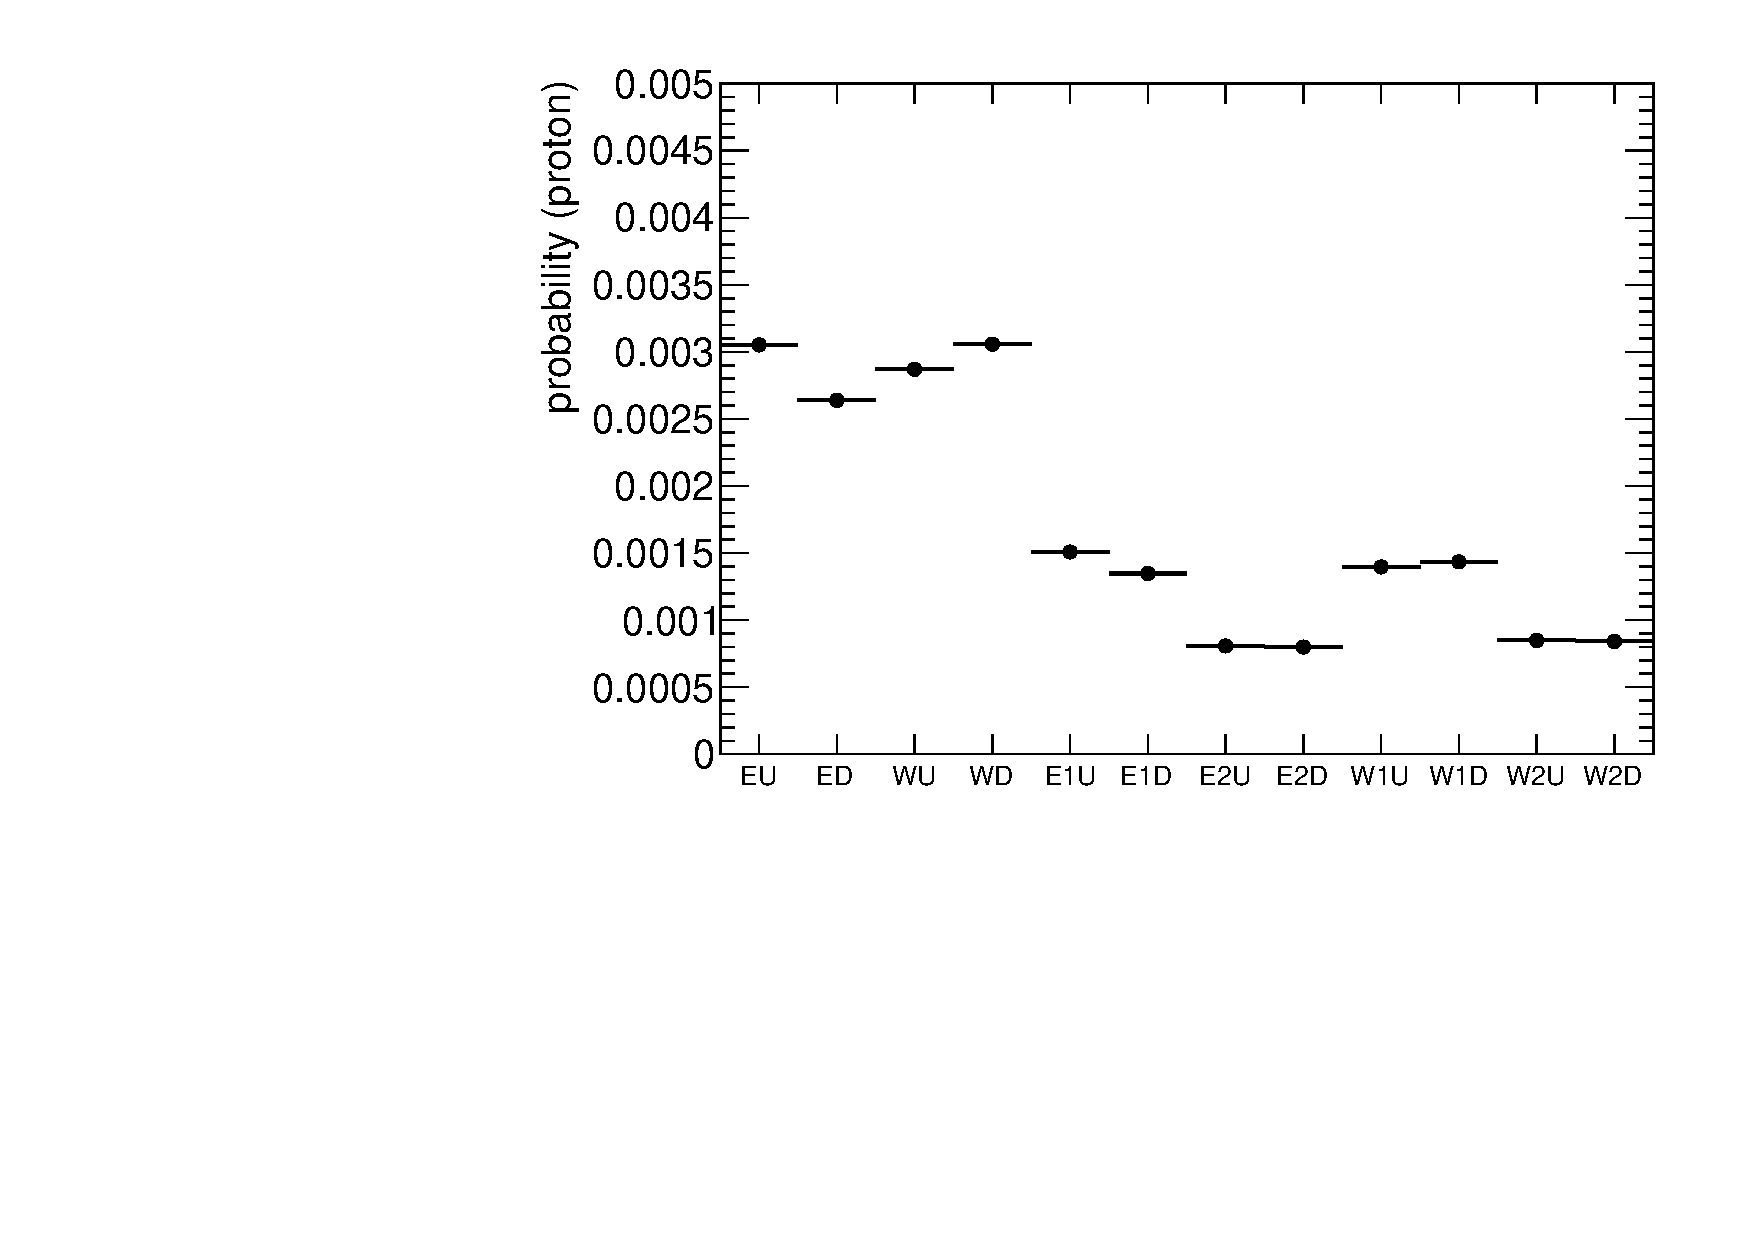
\includegraphics[width=\linewidth, page=1]{graphics/accidentals/accidentalBkg_1RP.pdf}}}
		\end{subfigure}
	}
	\quad
	\parbox{0.48\textwidth}{
		\centering
		\begin{subfigure}[b]{\linewidth}{
				\subcaptionbox{\label{fig:probCD}}{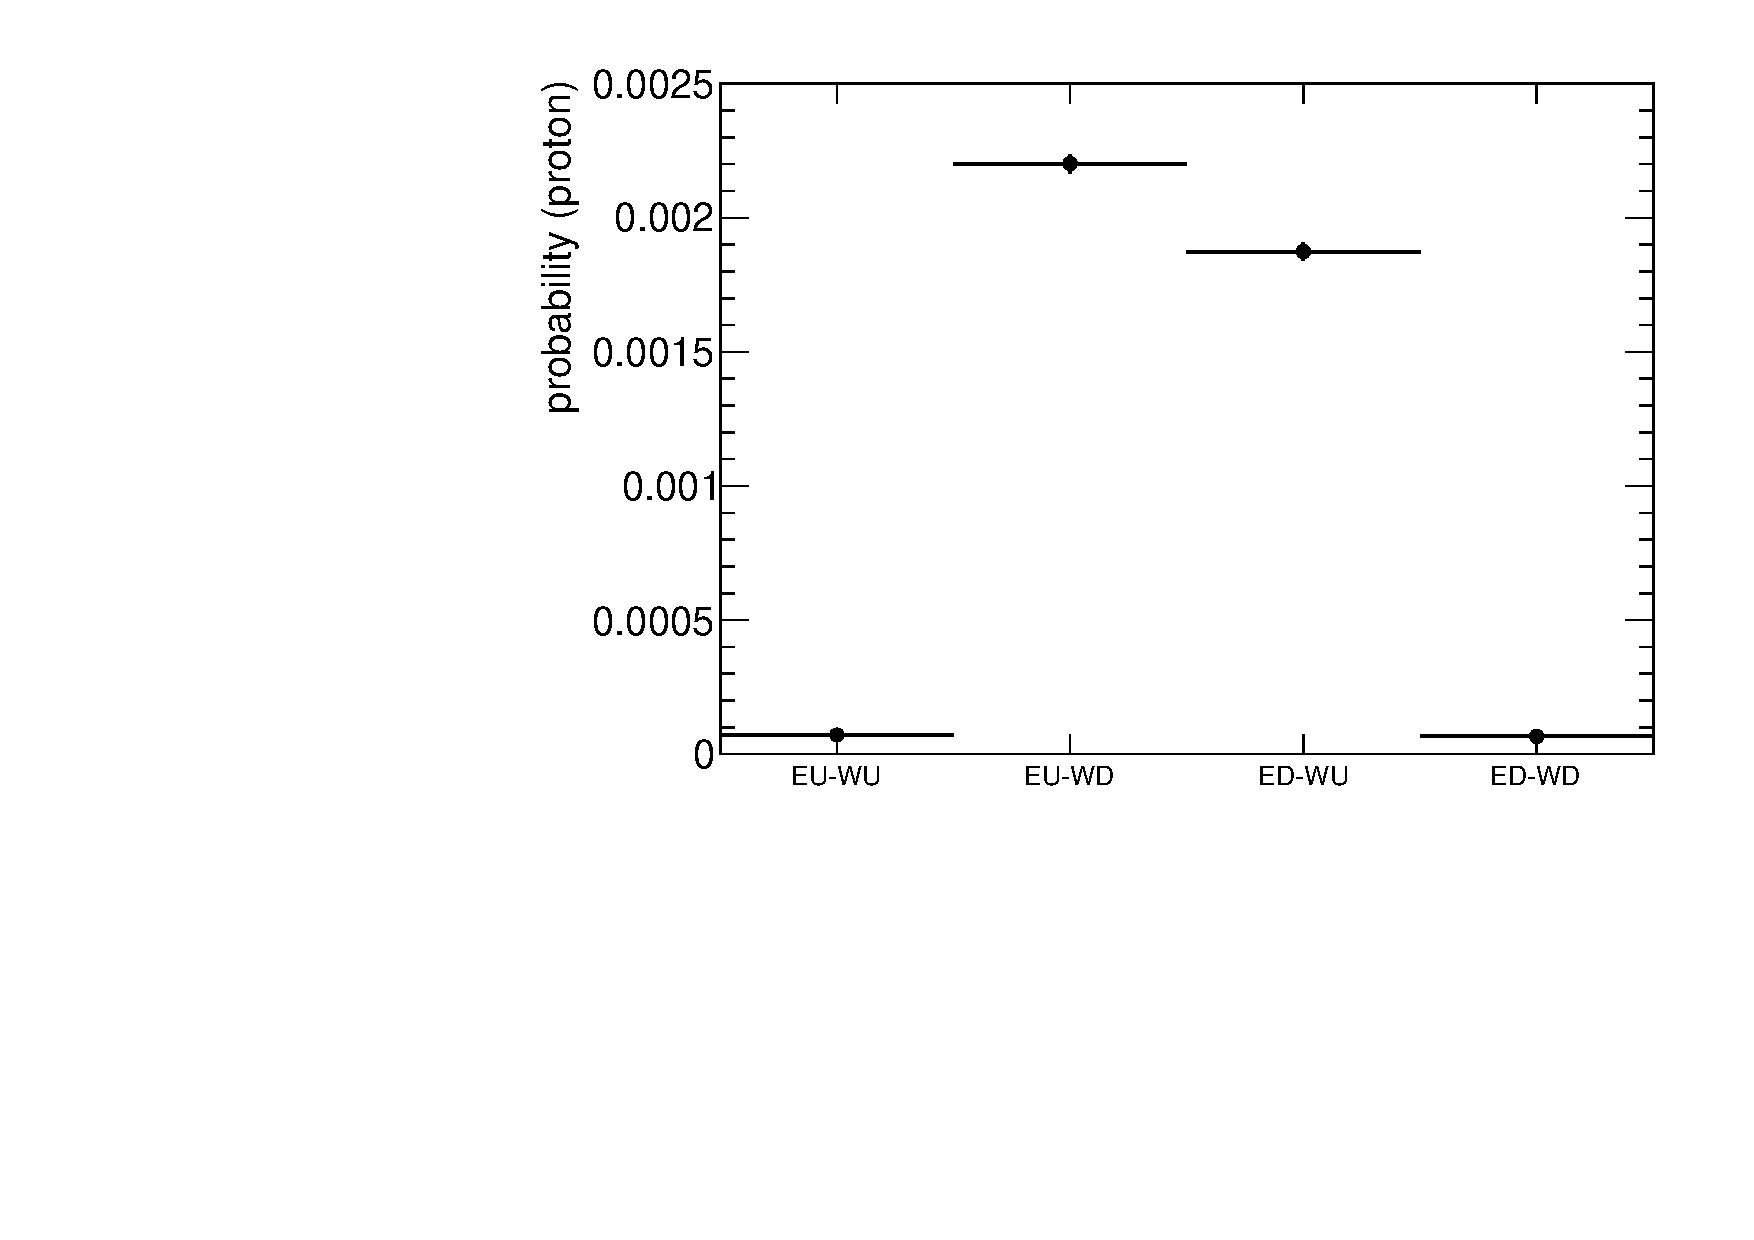
\includegraphics[width=\linewidth]{graphics/accidentals/accidentalBkg_2RP_cd.pdf}}}
		\end{subfigure}
	}%
	\caption[Proton overlay probability calculated from \textbf{Zerobias} trigger sample for SD and CD]{Proton overlay probability calculated from \textbf{Zerobias} trigger sample for SD (a) and CD (b, only proton global tracks used). The probability to observe accidental global tracks in RP in SD varies between $0.25-0.3\%$. Most of the accidental background in CD comes from the elastic RP configuration.}
	
	 %\label{fig:probacc}
\end{figure}
\subsection{Accidental background in SD}
The background from accidentals in SD events was calculated from the \textbf{Zerobias} sample multiplied by the probability of observing the accidental proton track in the RP and corrected by the relevant trigger prescales $\frac{PS^{Zerobias}}{PS^{SDT}}$. Figure \ref{fig:hitSD} shows the proton hit position in E1U with the data-driven background contribution for the region of interest (a,b - proton global and local tracks; c,d - only proton global tracks). 
\begin{figure}[H]
	\centering
	\parbox{0.48\textwidth}{
		\centering
		\begin{subfigure}[b]{\linewidth}{
				\subcaptionbox{\label{fig:E1UX}}{\includegraphics[width=\linewidth, page=14]{graphics/accidentals/accidentalBkg_1RP.pdf}}}
		\end{subfigure}
	}
	\quad
	\parbox{0.48\textwidth}{
		\centering
		\begin{subfigure}[b]{\linewidth}{
				\subcaptionbox{\label{fig:E1UY}}{\includegraphics[width=\linewidth, page=15]{graphics/accidentals/accidentalBkg_1RP.pdf}}}
		\end{subfigure}
	}
	\parbox{0.48\textwidth}{
		\centering
		\begin{subfigure}[b]{\linewidth}{
				\subcaptionbox{\label{fig:E1UglobalX}}{\includegraphics[width=\linewidth,page=14]{graphics/accidentals/accidentalBkg.pdf}}}
		\end{subfigure}
	}
	\quad
	\parbox{0.48\textwidth}{
		\centering
		\begin{subfigure}[b]{\linewidth}{
				\subcaptionbox{\label{fig:E1UglobalY}}{\includegraphics[width=\linewidth,page=15]{graphics/accidentals/accidentalBkg.pdf}}}
		\end{subfigure}
	}
	\caption[Proton hit position in SD using global+local proton tracks (a-b) and only global proton tracks]{Proton hit position in SD using global+local proton tracks (a-b) and only global proton tracks (c-d). The background contribution equals to about $10\%$.}
	 \label{fig:hitSD}
\end{figure}
Due to observe the same  accidental backround contribution  for global and global+local proton track $\left(\approx 10\%\right)$, also the $-t$ and $\xi$ distributions were checked (Figure \ref{fig:txiSD}). To reconstruct properly $-t$ and $\xi$ only global proton tracks were used. The flat background was observed in the $-t$ distribution. However, the $\xi$ distribution shows that most of the background is located around $\xi\approx 0$, which confirms the assumption that most of the accidental background comes from elastic, beam halo or low mass diffractive protons.
\begin{figure}[H]
	\centering
	\parbox{0.48\textwidth}{
		\centering
		\begin{subfigure}[b]{\linewidth}{
				\subcaptionbox{\label{fig:tSD}}{\includegraphics[width=\linewidth, page=33]{graphics/accidentals/accidentalBkg.pdf}}}
		\end{subfigure}
	}
	\quad
	\parbox{0.48\textwidth}{
		\centering
		\begin{subfigure}[b]{\linewidth}{
				\subcaptionbox{\label{fig:xiSD}}{\includegraphics[width=\linewidth, page=37]{graphics/accidentals/accidentalBkg.pdf}}}
		\end{subfigure}
	}
	\caption[$-t$ and $\xi$ distribution for WD arm in SD]{$-t$ and $\xi$ distribution for WD arm in SD. Accidental background suppressed for $0.02<\xi<0.4$.}
	 \label{fig:txiSD}
\end{figure}

 Additionally, the background begins to rise at $\xi\approx 0.4$. This probably comes from  true or fake tracks reconstructed in RP arising from showers happening outside the RP stations. Finally, the additional proton selection cuts were obtained for SD - the proton track is required to be a global track with $0.02 < \xi < 0.4$. The probability to observe the accidental proton in RP decreased to about $0.15\%$ (Figure \ref{fig:probSDcut}) and the accidental background contribution is about $5-10\%$ (Figure \ref{fig:tSDcut}).
 \begin{figure}[H]
 	\centering
 	\parbox{0.48\textwidth}{
 		\centering
 		\begin{subfigure}[b]{\linewidth}{
 				\subcaptionbox{\label{fig:probSDcut}}{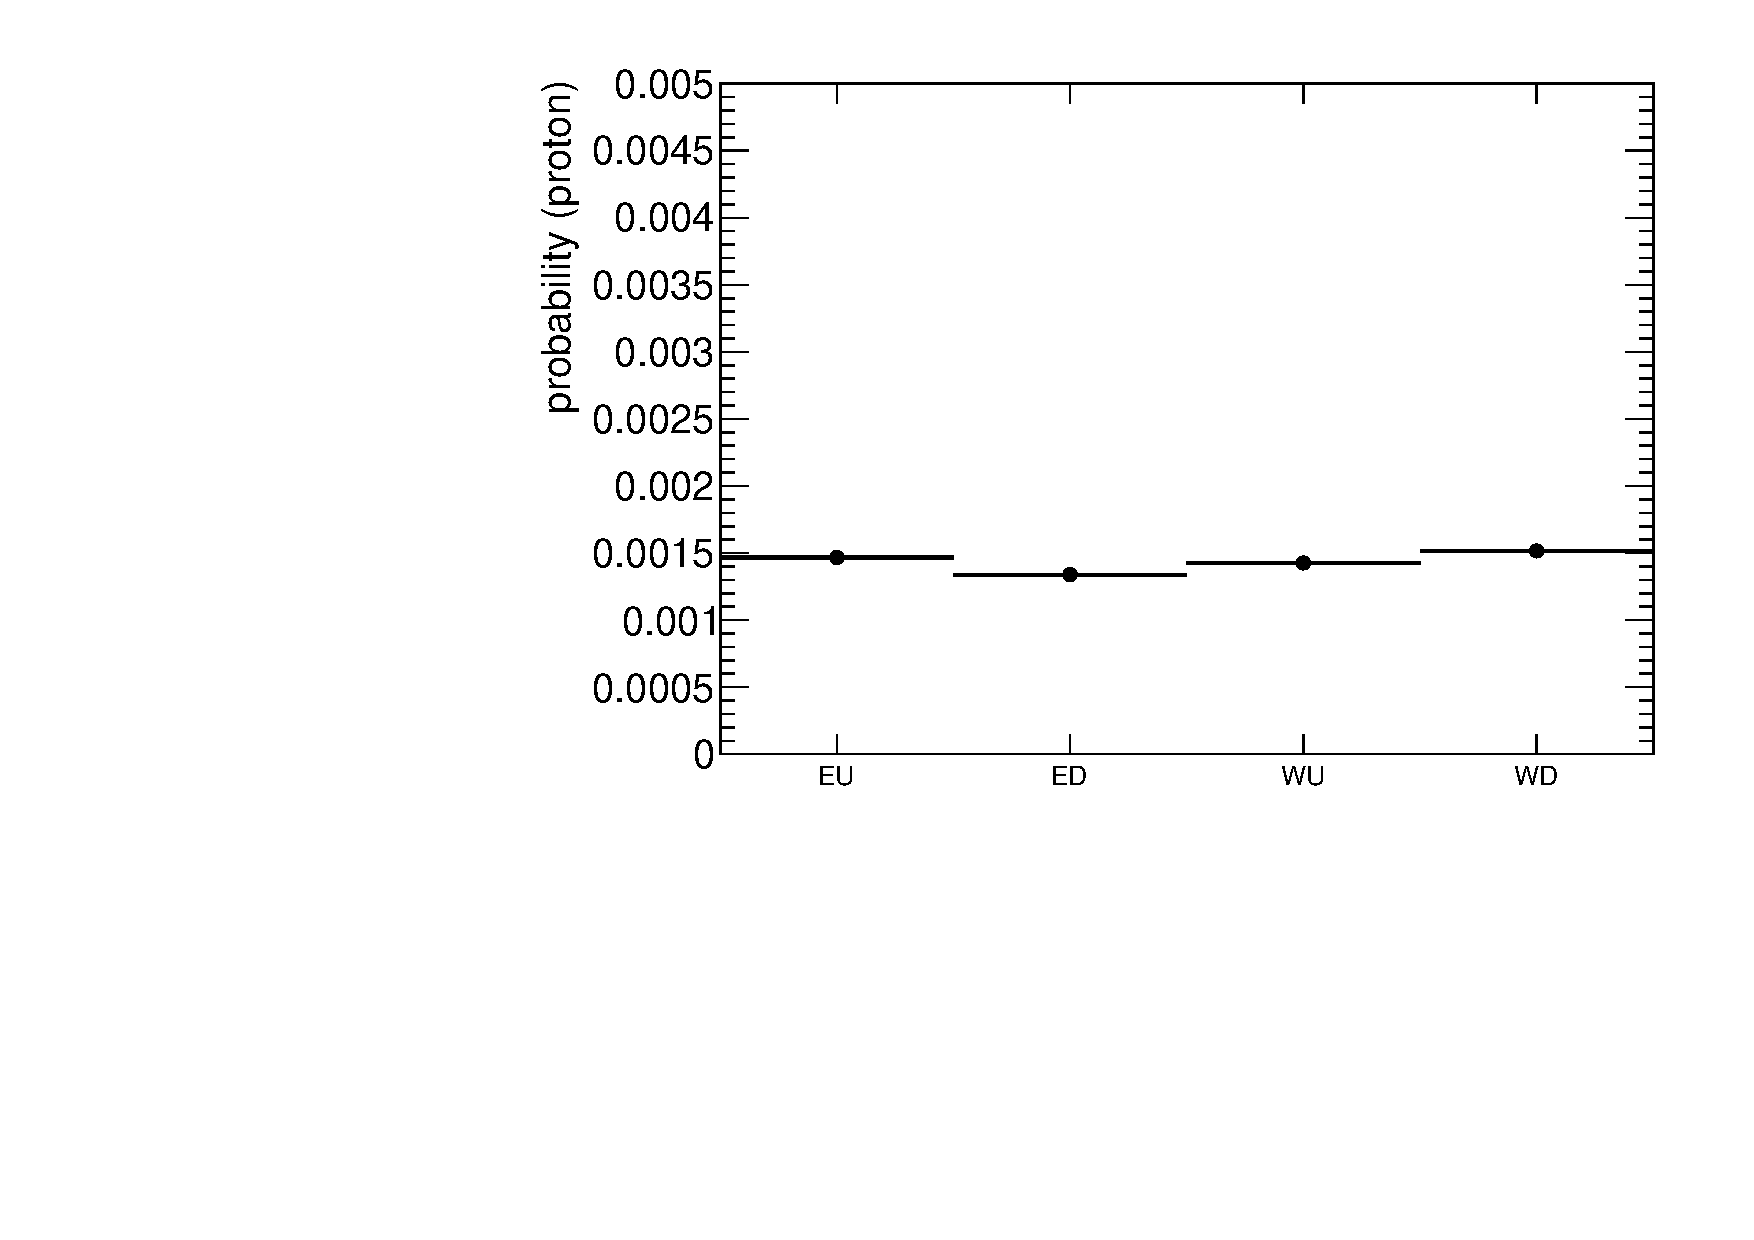
\includegraphics[width=\linewidth, page=1]{graphics/accidentals/accidentalBkg_XiCut2.pdf}}}
 		\end{subfigure}
 	}
 	\quad
 	\parbox{0.48\textwidth}{
 		\centering
 		\begin{subfigure}[b]{\linewidth}{
 				\subcaptionbox{\label{fig:tSDcut}}{\includegraphics[width=\linewidth, page=33]{graphics/accidentals/accidentalBkg_XiCut2.pdf}}}
 		\end{subfigure}
 	}
 	% \label{fig:xy_recoEff}
 	\caption[Proton overlay probability and $-t$ distribution for SD events with $0.02 < \xi < 0.4$]{Proton overlay probability (a) and $-t$ (b) distribution for SD events with $0.02 < \xi < 0.4$. The~probability to observe accidental proton in RP decreased to about $0.15\%$.}
 \end{figure}
 \begin{figure}[H]
 	\centering
 	\parbox{0.48\textwidth}{
 		\centering
 		\begin{subfigure}[b]{\linewidth}{
 				\subcaptionbox{\label{fig:xSDcut}}{\includegraphics[width=\linewidth, page=14]{graphics/accidentals/accidentalBkg_XiCut2.pdf}}}
 		\end{subfigure}
 	}
 	\quad
 	\parbox{0.48\textwidth}{
 		\centering
 		\begin{subfigure}[b]{\linewidth}{
 				\subcaptionbox{\label{fig:ySDcut}}{\includegraphics[width=\linewidth, page=15]{graphics/accidentals/accidentalBkg_XiCut2.pdf}}}
 		\end{subfigure}
 	}
 	\caption[Proton hit position in E1U for SD events with $0.02 < \xi < 0.4$.]{Proton hit position in E1U for SD events with $0.02 < \xi < 0.4$.}
 	% \label{fig:xy_recoEff}
 \end{figure}
 \begin{figure}[H]
 	\centering
 	\parbox{0.48\textwidth}{
 		\centering
 		\begin{subfigure}[b]{\linewidth}{
 				\subcaptionbox{\label{fig:ntrSDcut}}{\includegraphics[width=\linewidth, page=2]{graphics/accidentals/accidentalBkg_XiCut2.pdf}}}
 		\end{subfigure}
 	}
 	\quad
 	\parbox{0.48\textwidth}{
 		\centering
 		\begin{subfigure}[b]{\linewidth}{
 				\subcaptionbox{\label{fig:etaSDcut}}{\includegraphics[width=\linewidth, page=5]{graphics/accidentals/accidentalBkg_XiCut2.pdf}}}
 		\end{subfigure}
 	}
 	% \label{fig:xy_recoEff}
 	\caption[TPC-TOF related variables (TPC-TOF track multiplicity and $\eta$ of those tracks) for SD events with $0.02 < \xi < 0.4$.]{TPC-TOF related variables (TPC-TOF track multiplicity and $\eta$ of those tracks) for SD events with $0.02 < \xi < 0.4$. The background contribution is about $5-10\%$.}
 \end{figure}
 %\clearpage
 %\newpage
\subsection{Accidental background in CD}
The background from accidentals in CD events was calculated in the similar way to the SD. Only proton global tracks were used to calculate the probability of observing two accidental protons on the opposite sides of the IP. Figure \ref{fig:CDcoll} shows the collinearity distributions for inelastic (a) and elastic (b) RP configuration. 
\begin{figure}[H]
	\centering
	\parbox{0.48\textwidth}{
		\centering
		\begin{subfigure}[b]{\linewidth}{
				\subcaptionbox{\label{fig:accThetaX}}{\includegraphics[width=\linewidth, page=49]{graphics/accidentals/accidentalBkg_2RP_cd.pdf}}}
		\end{subfigure}
	}
	\quad
	\parbox{0.48\textwidth}{
		\centering
		\begin{subfigure}[b]{\linewidth}{
				\subcaptionbox{\label{fig:accThetaY}}{\includegraphics[width=\linewidth, page=55]{graphics/accidentals/accidentalBkg_2RP_cd.pdf}}}
		\end{subfigure}
	}
	\parbox{0.48\textwidth}{
		\centering
		\begin{subfigure}[b]{\linewidth}{
				\subcaptionbox{\label{fig:accTheta}}{\includegraphics[width=\linewidth, page=7]{graphics/accidentals/accidentalBkg_2RP_cd_scale.pdf}}}
		\end{subfigure}
	}
	% \label{fig:xy_recoEff}
	\caption[Collinearity distribution $\theta_X$ for inelastic and elastic RP configuration in CD]{Collinearity distribution $\theta_X$ for inelastic (a) and elastic (b) RP configuration in CD. The accidental background for elastic configuration is overestimated. The background was normalized to the signal in the first bin of the collinearity distribution (c).}
	\label{fig:CDcoll}
\end{figure}
The accidental background for the elastic configuration excess the $100\%$ and is overestimated. Two solutions were found to estimate the background in the elastic RP configuration:
\begin{enumerate}
	\item Require the protons to be anti-collinear $\left(\left(\delta\theta_x/\sigma_x\right)^2+\left(\delta\theta_y/\sigma_y\right)^2>3^2\right)$. 
\begin{figure}[H]
	\centering
	\parbox{0.48\textwidth}{
		\centering
		\begin{subfigure}[b]{\linewidth}{
				\subcaptionbox{\label{fig:accCDxiColl}}{\includegraphics[width=\linewidth, page=26]{graphics/accidentals/accidentalBkg_2RP_cd_Coll.pdf}}}
		\end{subfigure}
	}
	\quad
	\parbox{0.48\textwidth}{
		\centering
		\begin{subfigure}[b]{\linewidth}{
				\subcaptionbox{\label{fig:accCut}}{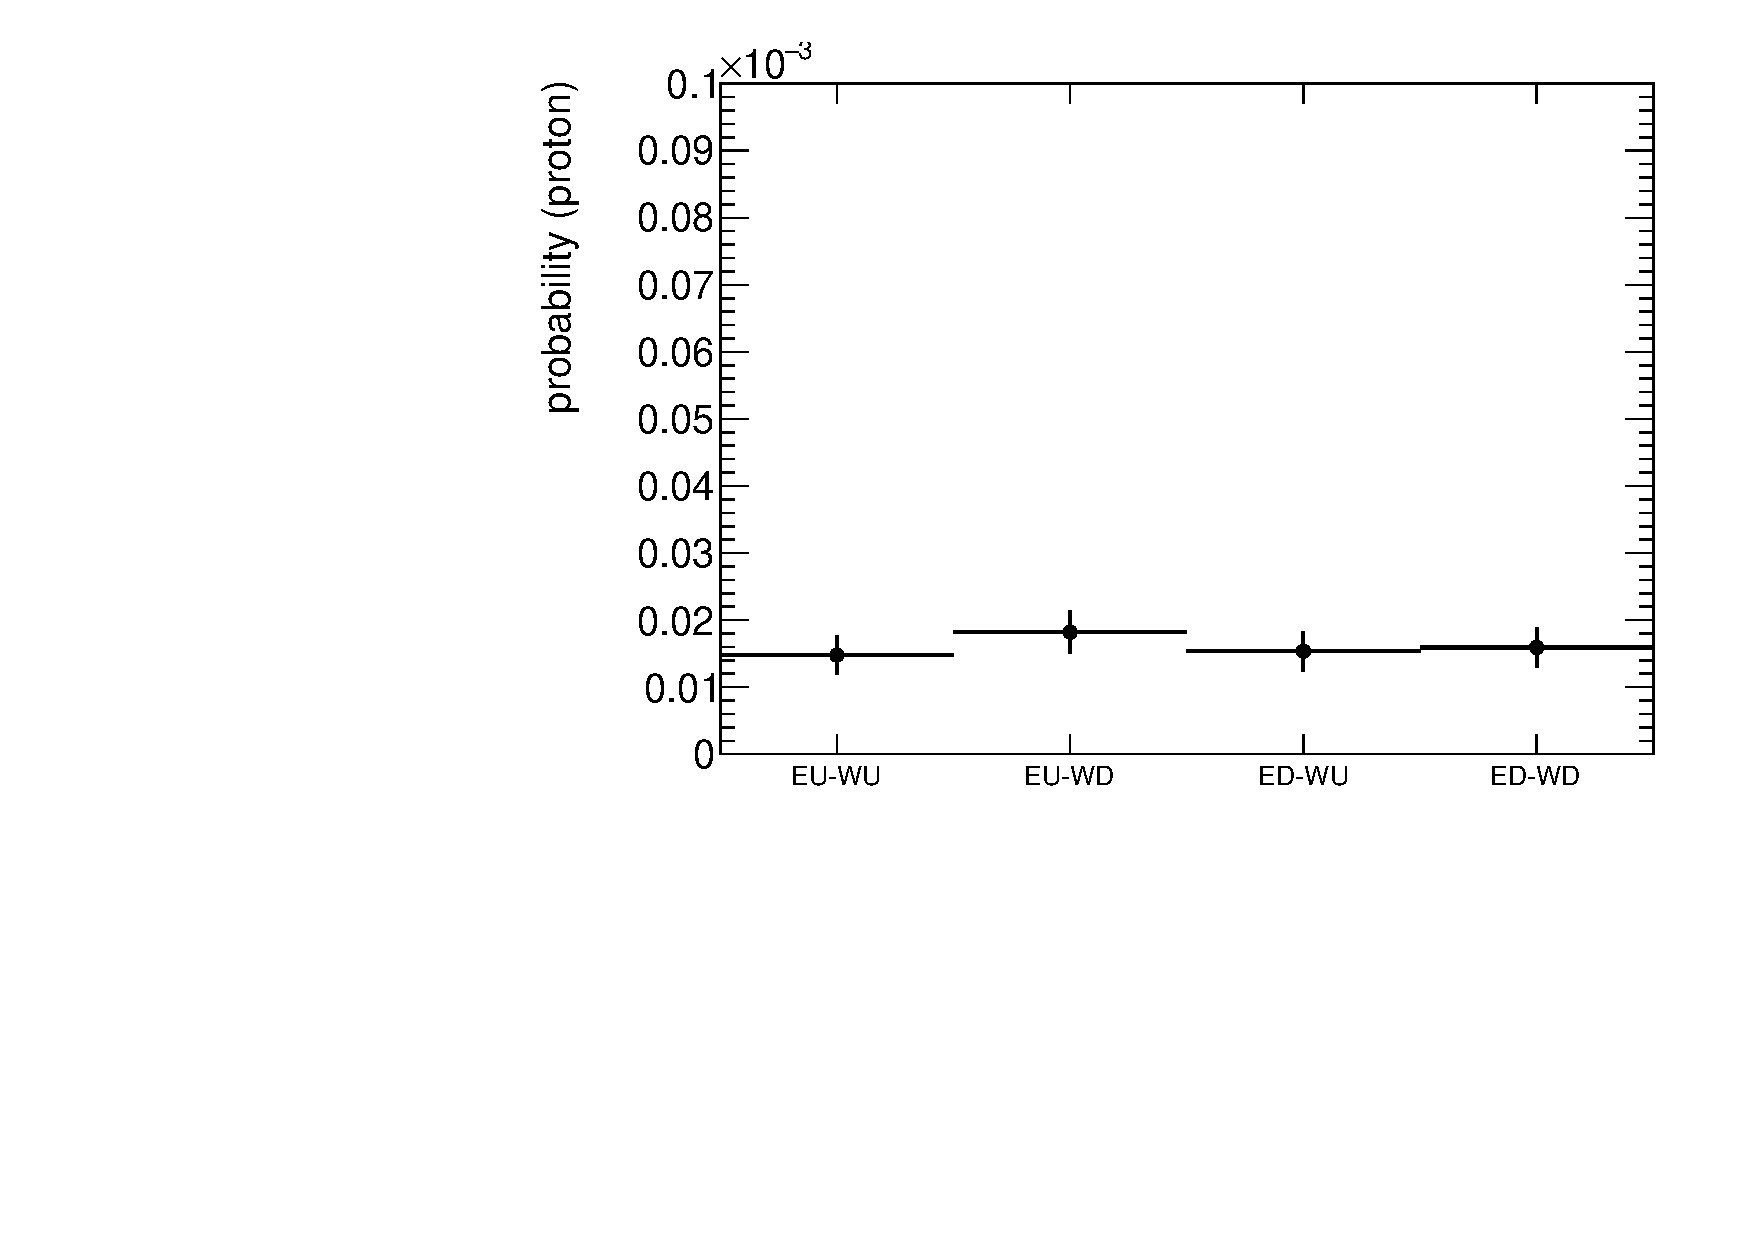
\includegraphics[width=\linewidth, page=1]{graphics/accidentals/accidentalBkg_2RP_cd_cut_NoColl.pdf}}}
		\end{subfigure}
	}
	\parbox{0.48\textwidth}{
		\centering
		\begin{subfigure}[b]{\linewidth}{
				\subcaptionbox{\label{fig:accThetaCut}}{\includegraphics[width=\linewidth, page=54]{graphics/accidentals/accidentalBkg_2RP_cd_cut_NoColl.pdf}}}
		\end{subfigure}
	}
	% \label{fig:xy_recoEff}
	\caption[x]{$\xi$ distribution of protons in EU arm with anti-collinearity cut. The background is suppressed for  $0.02<\xi_1,\xi_2<0.4$ and the proton overlay probability is reduced to $2\cdot10^{-5}$. The accidental background contribution was reduced to about $5\%$ with this cut.}
\end{figure}
	The $\xi$ distribution  with anti-collinearity cut, as shown in Figure \ref{fig:accCDxiColl}, was checked and it was found that the proton tracks should be required to be global tracks with $0.02<\xi_1,\xi_2<0.4$. With this cuts the probability of observing two accidental protons was reduced to about $2\cdot10^{-5}$ for all RP configurations (Figure \ref{fig:accCut}). Additionally, the overestimation of the background was not observed in the collinearity distribution (Figure \ref{fig:accThetaCut}) and the accidental background contribution decreased to about $5\%$.
\begin{figure}[H]
	\centering
	\parbox{0.48\textwidth}{
		\centering
		\begin{subfigure}[b]{\linewidth}{
				\subcaptionbox{\label{fig:accCDxielCut}}{\includegraphics[width=\linewidth, page=35]{graphics/accidentals/accidentalBkg_2RP_cd_cut_NoColl.pdf}}}
		\end{subfigure}
	}
	\quad
	\parbox{0.48\textwidth}{
		\centering
		\begin{subfigure}[b]{\linewidth}{
				\subcaptionbox{\label{fig:accCDtelCut}}{\includegraphics[width=\linewidth, page=43]{graphics/accidentals/accidentalBkg_2RP_cd_cut_NoColl.pdf}}}
		\end{subfigure}
	}
	\parbox{0.48\textwidth}{
		\centering
		\begin{subfigure}[b]{\linewidth}{
				\subcaptionbox{\label{fig:accCDxiinelCut}}{\includegraphics[width=\linewidth, page=33]{graphics/accidentals/accidentalBkg_2RP_cd_cut_NoColl.pdf}}}
		\end{subfigure}
	}
	\quad
	\parbox{0.48\textwidth}{
		\centering
		\begin{subfigure}[b]{\linewidth}{
				\subcaptionbox{\label{fig:accCDtinelCut}}{\includegraphics[width=\linewidth, page=41]{graphics/accidentals/accidentalBkg_2RP_cd_cut_NoColl.pdf}}}
		\end{subfigure}
	}
	% \label{fig:xy_recoEff}
	\caption[x]{$\xi$ and $-t$ in elastic and inelastic RP configuration measured with EU. The background is reduced to about $5\%$ in both RP configurations.}
\end{figure}
	\item Normalize the background to the signal in the first bin  of the collinearity distribution (Figure \ref{fig:accTheta}). Here it was assumed that all collinear protons are background protons and the upper limit for the background was set. Also the scale factor for the background was found. Similar to the first method, it was found that the background is supressed for $0.02<\xi_1,\xi_2<0.4$ and varies between $2-3\%$ (Figure \ref{fig:xecCutAcc} b-d). The collinearity cut is not required anymore.
\begin{figure}[H]
	\centering
	\parbox{0.48\textwidth}{
		\centering
		\begin{subfigure}[b]{\linewidth}{
				\subcaptionbox{\label{fig:accCDxiel2}}{\includegraphics[width=\linewidth, page=30]{graphics/accidentals/accidentalBkg_2RP_cd_scale.pdf}}}
		\end{subfigure}
	}
	\quad
	\parbox{0.48\textwidth}{
		\centering
		\begin{subfigure}[b]{\linewidth}{
				\subcaptionbox{\label{fig:accCDxiCut2}}{\includegraphics[width=\linewidth, page=30]{graphics/accidentals/accidentalBkg_2RP_cd_Cut_scale.pdf}}}
		\end{subfigure}
	}
	\parbox{0.48\textwidth}{
		\centering
		\begin{subfigure}[b]{\linewidth}{
				\subcaptionbox{\label{fig:accCDtelCut2}}{\includegraphics[width=\linewidth, page=38]{graphics/accidentals/accidentalBkg_2RP_cd_Cut_scale.pdf}}}
		\end{subfigure}
	}
	\quad
	\parbox{0.48\textwidth}{
		\centering
		\begin{subfigure}[b]{\linewidth}{
				\subcaptionbox{\label{fig:accCDCollCut2}}{\includegraphics[width=\linewidth, page=4]{graphics/accidentals/accidentalBkg_2RP_cd_Cut_scale.pdf}}}
		\end{subfigure}
	}
	% \label{fig:xy_recoEff}
	\caption[x]{$\xi$ distribution in CD with the accidental background normalized to the signal in the first bin of the collinearity distribution (Figure \ref{fig:accTheta}). Most of the accidental background located outside the $0.02<\xi_1,\xi_2<0.4$ region. The background reduced to about $2-3\%$ in $\xi$, $-t$ and collinearity distributions with $0.02<\xi_1,\xi_2<0.4$ cut applied.}
	\label{fig:xecCutAcc}
\end{figure}
\end{enumerate}
\begin{figure}[H]
	\centering
	\parbox{0.48\textwidth}{
		\centering
		\begin{subfigure}[b]{\linewidth}{
				\subcaptionbox{\label{fig:accCDxin}}{\includegraphics[width=\linewidth, page=61]{graphics/accidentals/accidentalBkg_2RP_cd_cut_NoColl.pdf}}}
		\end{subfigure}
	}
	\quad
	\parbox{0.48\textwidth}{
		\centering
		\begin{subfigure}[b]{\linewidth}{
				\subcaptionbox{\label{fig:accCDyin}}{\includegraphics[width=\linewidth, page=62]{graphics/accidentals/accidentalBkg_2RP_cd_cut_NoColl.pdf}}}
		\end{subfigure}
	}
	\parbox{0.48\textwidth}{
		\centering
		\begin{subfigure}[b]{\linewidth}{
				\subcaptionbox{\label{fig:accCDxel}}{\includegraphics[width=\linewidth, page=69]{graphics/accidentals/accidentalBkg_2RP_cd_cut_NoColl.pdf}}}
		\end{subfigure}
	}
	\quad
	\parbox{0.48\textwidth}{
		\centering
		\begin{subfigure}[b]{\linewidth}{
				\subcaptionbox{\label{fig:accCDyel}}{\includegraphics[width=\linewidth, page=70]{graphics/accidentals/accidentalBkg_2RP_cd_cut_NoColl.pdf}}}
		\end{subfigure}
	}
	% \label{fig:xy_recoEff}
	\caption[x]{Proton hit positions for E2U in inelastic (a, b) and elastic (c,d) RP configuration with $0.02<\xi_1,\xi_2<0.4$ cut applied. The background reduced to about $2-4\%$ in both RP configurations.}
\end{figure}
\begin{figure}[H]
	\centering
	\parbox{0.48\textwidth}{
		\centering
		\begin{subfigure}[b]{\linewidth}{
				\subcaptionbox{\label{fig:accCDntrinel}}{\includegraphics[width=\linewidth, page=12]{graphics/accidentals/accidentalBkg_2RP_cd_Cut_scale.pdf}}}
		\end{subfigure}
	}
	\quad
	\parbox{0.48\textwidth}{
		\centering
		\begin{subfigure}[b]{\linewidth}{
				\subcaptionbox{\label{fig:accCDetael}}{\includegraphics[width=\linewidth, page=24]{graphics/accidentals/accidentalBkg_2RP_cd_Cut_scale.pdf}}}
		\end{subfigure}
	}
	\parbox{0.48\textwidth}{
		\centering
		\begin{subfigure}[b]{\linewidth}{
				\subcaptionbox{\label{fig:accCDntrel}}{\includegraphics[width=\linewidth, page=13]{graphics/accidentals/accidentalBkg_2RP_cd_Cut_scale.pdf}}}
		\end{subfigure}
	}
	\quad
	\parbox{0.48\textwidth}{
		\centering
		\begin{subfigure}[b]{\linewidth}{
				\subcaptionbox{\label{fig:accCDetainel}}{\includegraphics[width=\linewidth, page=25]{graphics/accidentals/accidentalBkg_2RP_cd_Cut_scale.pdf}}}
		\end{subfigure}
	}
	% \label{fig:xy_recoEff}
	\caption[x]{TPC-TOF related variables (TPC-TOF track multiplicity and $\eta$ of those tracks) for CD events with $0.02<\xi_1,\xi_2<0.4$. The background contribution is about $0.5\%$.}
\end{figure}

\subsection{TPC related distributions with additional proton selection cuts}
The additional proton selection $\xi\left(\xi_1,\xi_2\right)$ cuts reduce the statistics of about $20\%$ and $50\%$ for SD and CD, respectively. The most significant background reduction was observed mainly in CD. Figure \ref{fig:reduction} shows the comparison of the $p_T$ (c, f) and $\eta$ (b, e) distibutions with and without the $\xi\left(\xi_1,\xi_2\right)$ cuts applied. In spite of the reduction of the background, the shape of those distributions did not change. Although, the TPC-TOF track multiplicity distribution changed with above cuts applied (Figure \ref{fig:reduction} a, d). The rest of the accidental background has to be  subtracted statistically.
\begin{figure}[H]
	\centering
	\parbox{0.31\textwidth}{
		\centering
		\begin{subfigure}[b]{\linewidth}{
				\subcaptionbox{\label{fig:redSDntr}}{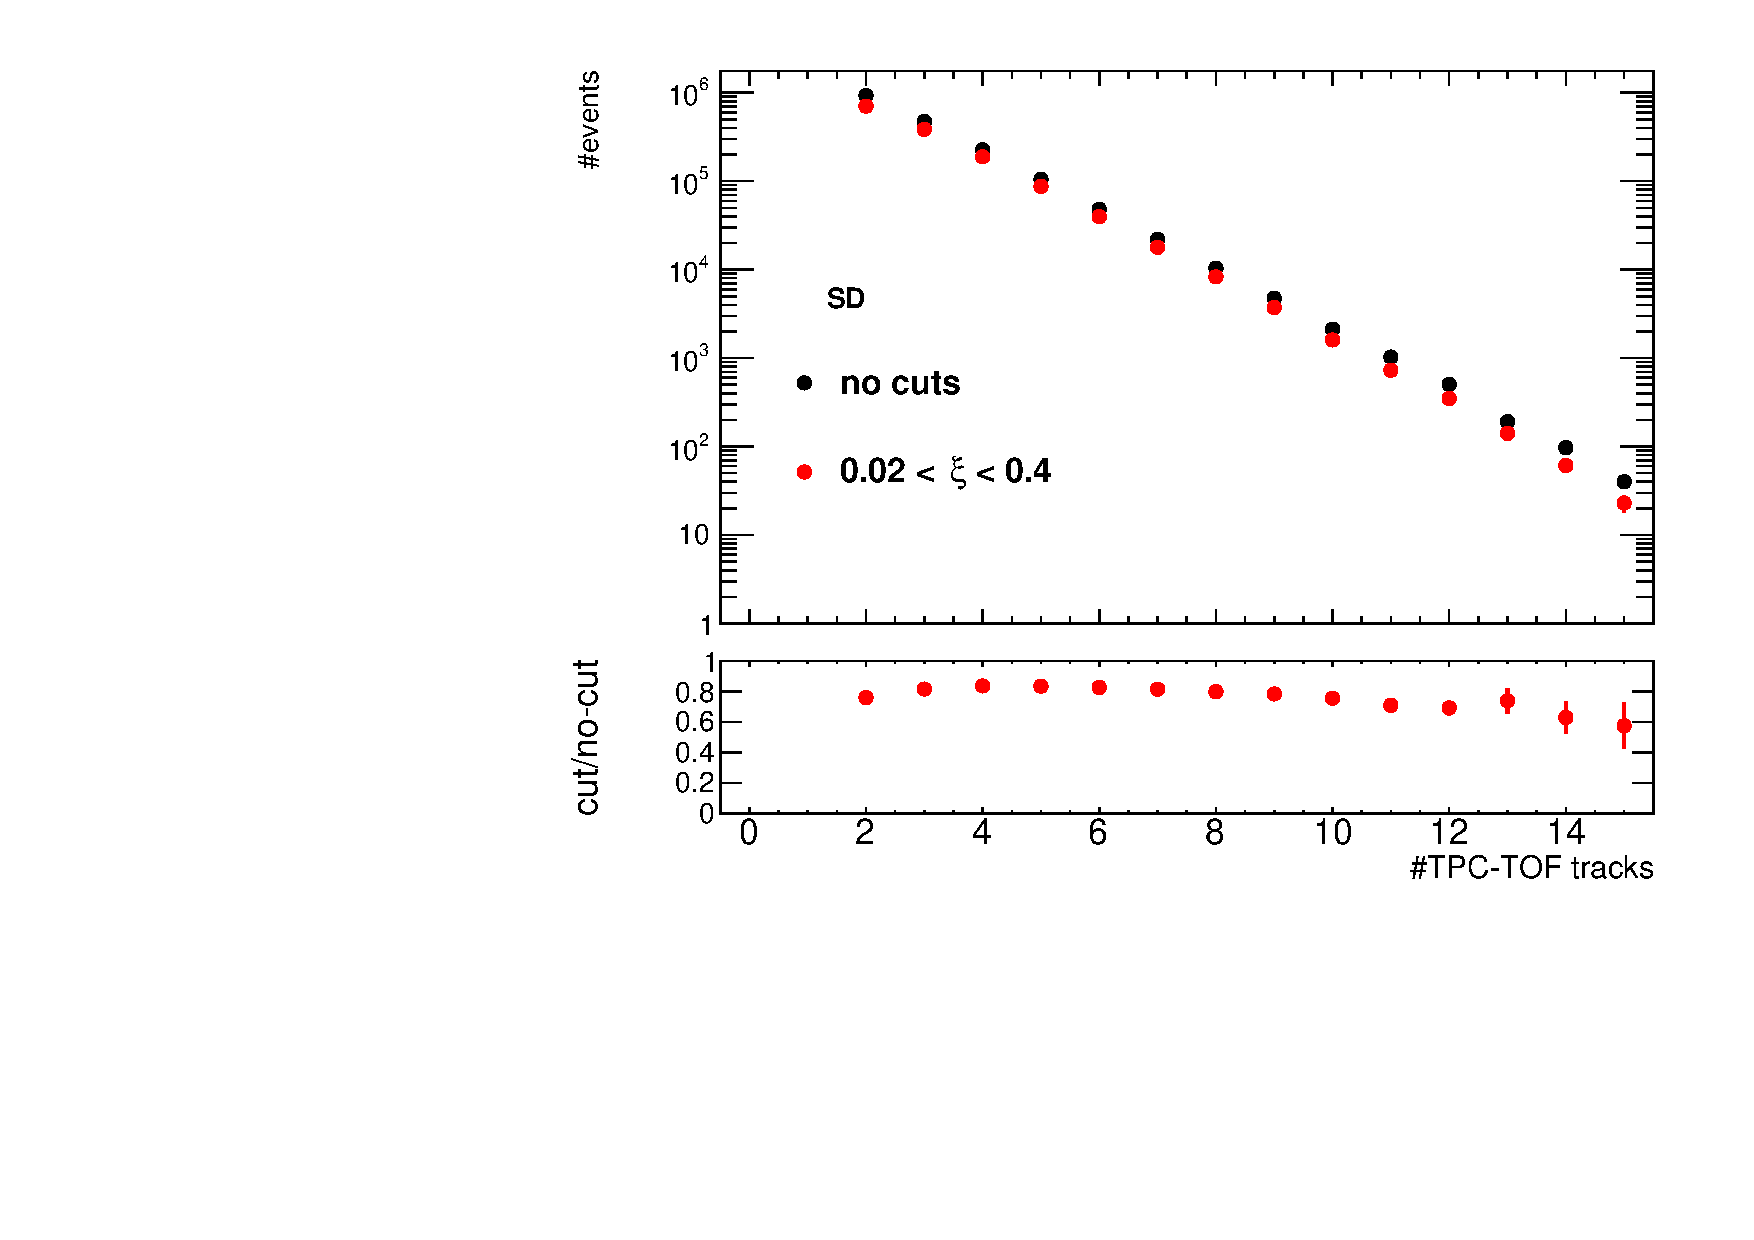
\includegraphics[width=\linewidth, page=1]{graphics/accidentals/compareCuts.pdf}}}
		\end{subfigure}
	}
	\quad
	\parbox{0.31\textwidth}{
		\centering
		\begin{subfigure}[b]{\linewidth}{
				\subcaptionbox{\label{fig:redSDeta}}{\includegraphics[width=\linewidth, page=3]{graphics/accidentals/compareCuts.pdf}}}
		\end{subfigure}
	}
	\quad
	\parbox{0.31\textwidth}{
		\centering
		\begin{subfigure}[b]{\linewidth}{
				\subcaptionbox{\label{fig:redSDpt}}{\includegraphics[width=\linewidth, page=5]{graphics/accidentals/compareCuts.pdf}}}
		\end{subfigure}
	}
	\parbox{0.31\textwidth}{
		\centering
		\begin{subfigure}[b]{\linewidth}{
				\subcaptionbox{\label{fig:redCDntr}}{\includegraphics[width=\linewidth, page=2]{graphics/accidentals/compareCuts.pdf}}}
		\end{subfigure}
	}
	\quad
	\parbox{0.31\textwidth}{
		\centering
		\begin{subfigure}[b]{\linewidth}{
				\subcaptionbox{\label{fig:redCDeta}}{\includegraphics[width=\linewidth, page=4]{graphics/accidentals/compareCuts.pdf}}}
		\end{subfigure}
	}
	\quad
	\parbox{0.31\textwidth}{
		\centering
		\begin{subfigure}[b]{\linewidth}{
				\subcaptionbox{\label{fig:redCDpt}}{\includegraphics[width=\linewidth, page=6]{graphics/accidentals/compareCuts.pdf}}}
		\end{subfigure}
	}
   
	\caption[TPC-TOF related distributions with and without additional proton track selection cuts applied in SD and CD]{TPC-TOF related distributions with and without additional proton track selection cuts applied in SD (a-c) and CD (d-f). The additional proton selection $\xi\left(\xi_1,\xi_2\right)$ cuts reduce the statistics of about $20\%$ and $50\%$ for SD and CD, respectively.}
	\label{fig:reduction}
\end{figure}
\section{Corrections}\label{sec:Corrections}
\subsection{Monte Carlo Embedding Technique}
The correction factors are obtained by the multistep
embedding MC technique. First, simulated tracks are
blended into real events at the raw data level. Real data
events to be used in the embedding are sampled over the
entire data-taking period in order to have proper representation
of the whole data set used in the analysis.  Three samples of embedding MC were produced:
\begin{enumerate}
	\item The MC track kinematics are taken
	from flat distributions in $\eta$ and $p_T$. The flat $p_T$ distribution
	is used in order to have similar statistics in different
	$p_T$ bins.
	\item PYTHIA 8.186 SD  with Sch{\"u}ler and Sj{\"o}strand Pomeron Flux model (\cite{pythia8}).
	\item PYTHIA 8.186 CD  with Minimum Bias Rockefeller Pomeron Flux model (\cite{pythia8}).
\end{enumerate}
The tracks are propagated through the full simulation of
the STAR detector and geometry using GEANT with a
realistic simulation of the STAR-TPC response. The obtained raw data 
information for the simulated particles are added on to
the existing information of the real data. Next, the mixed events are treated just as real data
and are processed through the full reconstruction chain.

\subsection{Data-MC comparison}
\begin{figure}[H]
	\centering
	\parbox{0.484\textwidth}{
		\centering
		\begin{subfigure}[b]{\linewidth}{
				\subcaptionbox{\label{fig:cutFlownpra}}{\includegraphics[width=\linewidth, page=9]{graphics/cutFlow/SDT.pdf}}}
		\end{subfigure}
	}
	\quad
	\parbox{0.484\textwidth}{
		\centering
		\begin{subfigure}[b]{\linewidth}{
				\subcaptionbox{\label{fig:cutFlownprb}}{\includegraphics[width=\linewidth, page=7]{graphics/cutFlow/CPT2.pdf}}}
		\end{subfigure}
	}
	\caption[...]{...}
	\label{fig:cutFlownpr}
\end{figure}
\begin{figure}[H]
	\centering
	\parbox{0.484\textwidth}{
		\centering
		\begin{subfigure}[b]{\linewidth}{
				\subcaptionbox{\label{fig:cutFlowvza}}{\includegraphics[width=\linewidth, page=8]{graphics/cutFlow/SDT.pdf}}}
		\end{subfigure}
	}
	\quad
	\parbox{0.484\textwidth}{
		\centering
		\begin{subfigure}[b]{\linewidth}{
				\subcaptionbox{\label{fig:cutFlowvzb}}{\includegraphics[width=\linewidth, page=6]{graphics/cutFlow/CPT2.pdf}}}
		\end{subfigure}
	}
	\caption[...]{...}
	\label{fig:cutFlowvz}
\end{figure}
\begin{figure}[H]
	\centering
	\parbox{0.484\textwidth}{
		\centering
		\begin{subfigure}[b]{\linewidth}{
				\subcaptionbox{\label{fig:cutFlowEtaa}}{\includegraphics[width=\linewidth, page=2]{graphics/cutFlow/SDT.pdf}}}
		\end{subfigure}
	}
	\quad
	\parbox{0.484\textwidth}{
		\centering
		\begin{subfigure}[b]{\linewidth}{
				\subcaptionbox{\label{fig:cutFlowEtab}}{\includegraphics[width=\linewidth, page=2]{graphics/cutFlow/CPT2.pdf}}}
		\end{subfigure}
	}
	\caption[...]{...}
	\label{fig:cutFlowEta}
\end{figure}
\begin{figure}[H]
	\centering
	\parbox{0.484\textwidth}{
		\centering
		\begin{subfigure}[b]{\linewidth}{
				\subcaptionbox{\label{fig:cutFlowSDetaa}}{\includegraphics[width=\linewidth, page=3]{graphics/cutFlow/SDT.pdf}}}
		\end{subfigure}
	}
	\quad
	\parbox{0.484\textwidth}{
		\centering
		\begin{subfigure}[b]{\linewidth}{
				\subcaptionbox{\label{fig:cutFlowSDetab}}{\includegraphics[width=\linewidth, page=4]{graphics/cutFlow/SDT.pdf}}}
		\end{subfigure}
	}
	\caption[...]{...}
	\label{fig:cutFlowSDeta}
\end{figure}

\begin{figure}[H]
	\centering
	\parbox{0.484\textwidth}{
		\centering
		\begin{subfigure}[b]{\linewidth}{
				\subcaptionbox{\label{fig:cutFlowpta}}{\includegraphics[width=\linewidth, page=5]{graphics/cutFlow/SDT.pdf}}}
		\end{subfigure}
	}
	\quad
	\parbox{0.484\textwidth}{
		\centering
		\begin{subfigure}[b]{\linewidth}{
				\subcaptionbox{\label{fig:cutFlowptb}}{\includegraphics[width=\linewidth, page=3]{graphics/cutFlow/CPT2.pdf}}}
		\end{subfigure}
	}
	\caption[...]{...}
	\label{fig:cutFlowpt}
\end{figure}

\begin{figure}[H]
	\centering
	\parbox{0.484\textwidth}{
		\centering
		\begin{subfigure}[b]{\linewidth}{
				\subcaptionbox{\label{fig:cutFlowdcaa}}{\includegraphics[width=\linewidth, page=6]{graphics/cutFlow/SDT.pdf}}}
		\end{subfigure}
	}
	\quad
	\parbox{0.484\textwidth}{
		\centering
		\begin{subfigure}[b]{\linewidth}{
				\subcaptionbox{\label{fig:cutFlowdcab}}{\includegraphics[width=\linewidth, page=4]{graphics/cutFlow/CPT2.pdf}}}
		\end{subfigure}
	}
	\parbox{0.484\textwidth}{
		\centering
		\begin{subfigure}[b]{\linewidth}{
				\subcaptionbox{\label{fig:cutFlowdcac}}{\includegraphics[width=\linewidth, page=7]{graphics/cutFlow/SDT.pdf}}}
		\end{subfigure}
	}
	\quad
	\parbox{0.484\textwidth}{
		\centering
		\begin{subfigure}[b]{\linewidth}{
				\subcaptionbox{\label{fig:cutFlowdcad}}{\includegraphics[width=\linewidth, page=5]{graphics/cutFlow/CPT2.pdf}}}
		\end{subfigure}
	}	
	\caption[...]{...}
	\label{fig:cutFlowdca}
\end{figure}

\begin{figure}[H]
	\centering
	\parbox{0.484\textwidth}{
		\centering
		\begin{subfigure}[b]{\linewidth}{
				\subcaptionbox{\label{fig:cutFlowhitsa}}{\includegraphics[width=\linewidth, page=10]{graphics/cutFlow/SDT.pdf}}}
		\end{subfigure}
	}
	\quad
	\parbox{0.484\textwidth}{
		\centering
		\begin{subfigure}[b]{\linewidth}{
				\subcaptionbox{\label{fig:cutFlowhitsb}}{\includegraphics[width=\linewidth, page=8]{graphics/cutFlow/CPT2.pdf}}}
		\end{subfigure}
	}
	\parbox{0.484\textwidth}{
		\centering
		\begin{subfigure}[b]{\linewidth}{
				\subcaptionbox{\label{fig:cutFlowhitsc}}{\includegraphics[width=\linewidth, page=11]{graphics/cutFlow/SDT.pdf}}}
		\end{subfigure}
	}
	\quad
	\parbox{0.484\textwidth}{
		\centering
		\begin{subfigure}[b]{\linewidth}{
				\subcaptionbox{\label{fig:cutFlowhitsd}}{\includegraphics[width=\linewidth, page=9]{graphics/cutFlow/CPT2.pdf}}}
		\end{subfigure}
	}	
	\caption[...]{...}
	\label{fig:cutFlowhits}
\end{figure}

\subsection{Vertex reconstruction}
In $pp$ collisions, where the charged-particle multiplicity is low, the vertex finding algorithm sometimes fails to find a primary vertex. In addition, at high luminosity, vertex finder can fail due to the contribution of pile-up events and providing a wrong reconstructed vertex. In this study we require at least two reconstructed global tracks $N^{global}_{reco}\geq 2$ passing all the quality cuts listed in Table \ref{tab:trackCut} but without $\textrm{DCA}_{xy}$ and $\textrm{DCA}_{z}$ cuts. 

\subsubsection{Track quality cuts used for vertexing}
The tracks used by vertex finder have to  pass different set of quality cuts than used in this analysis. 
A global track $N^{global}_{vrt}$ used in vertex reconstruction has to pass the quality cuts listed in the Table \ref{tab:trackCutVertex}. Since that, vertex reconstruction efficiency and fake vertex rate is calculated as a function of $N^{global}_{vrt}$ instead of $N^{global}_{reco}$. 


\begin{table}[H]
	\centering
	\begin{tabular}{| l | l |}
		\hline			
		Quantity & Cut \\
		\hline
		\hline
		Number of Fit Points & Fit Points $>20$\\
		Transverse Impact Parameter & $|d_0|<2$~cm\\ 
		Ratio of Fit Points / Possible Fit Points & Fit Points/ Possible Fit Points $>0.52$\\
		Global Track Transverse Momentum & $p_{T}>0.2$~GeV/c\\
		TOF Matched Track & TOF Match-Flag $\geq1$\\
		\hline  
	\end{tabular}
	\caption[Vertexing Track Level Cuts]{Vertexing Track Level Cuts}
	\label{tab:trackCutVertex}
\end{table}
\subsubsection{Vertex efficiency and fake vertex}



\chapter{Systematic uncertainty study}\label{chap:SystematicStudy}
\chapter{Results}\label{chap:Results}


% %% ===== DODATKI ===== ------------
% \begin{appendices}
% \input{Appendix_RunList.tex}
% \input{Appendix_tDistributions.tex}
% \input{Appendix_AngularBeamDivergence.tex}
% \input{Appendix_BunchProfiles.tex}
% \end{appendices}
% %% ===== DODATKI ===== ------------
\begin{appendices}
\makeatletter
\renewcommand{\@makechapterhead}[1]{%
 \vspace*{-18\p@}%
  {\parindent \z@ \raggedright
%     \LARGE \bfseries \thechapter. #1\par\nobreak
%     \vskip 40\p@
      \Huge \bfseries Appendix \thechapter\newline #1\par\nobreak
      \vskip 20\p@
  }}
\makeatother

% %% =====  DEDX FITS ====
%%===========================================================%%
%%                                                           %%
%%              DEDX FITS APPENDIX            	%%
%%                                                           %%
%%===========================================================%%

\chapter{Distributions of $n\sigma^{i}_{dE/dx}$ in SD}\label{appendix:dEdxFits}

\begin{figure}[H]
	\centering
	\parbox{0.3\textwidth}{
		\centering
		\begin{subfigure}[b]{\linewidth}{
				{\includegraphics[width=\linewidth, page=2]{graphics/pid/spectraFit_SDT.pdf}}}
		\end{subfigure}
	}
	\quad
	\parbox{0.3\textwidth}{
		\centering
		\begin{subfigure}[b]{\linewidth}{
				{\includegraphics[width=\linewidth, page=3]{graphics/pid/spectraFit_SDT.pdf}}}
		\end{subfigure}
	}
	\parbox{0.3\textwidth}{
			\centering
			\begin{subfigure}[b]{\linewidth}{
					{\includegraphics[width=\linewidth, page=4]{graphics/pid/spectraFit_SDT.pdf}}}
			\end{subfigure}
		}
	\parbox{0.3\textwidth}{
		\centering
		\begin{subfigure}[b]{\linewidth}{
				{\includegraphics[width=\linewidth, page=5]{graphics/pid/spectraFit_SDT.pdf}}}
		\end{subfigure}
	}
	\quad
	\parbox{0.3\textwidth}{
		\centering
		\begin{subfigure}[b]{\linewidth}{
				{\includegraphics[width=\linewidth, page=6]{graphics/pid/spectraFit_SDT.pdf}}}
		\end{subfigure}
	}
	\parbox{0.3\textwidth}{
			\centering
			\begin{subfigure}[b]{\linewidth}{
					{\includegraphics[width=\linewidth, page=7]{graphics/pid/spectraFit_SDT.pdf}}}
			\end{subfigure}
		}
	\parbox{0.3\textwidth}{
		\centering
		\begin{subfigure}[b]{\linewidth}{
				{\includegraphics[width=\linewidth, page=8]{graphics/pid/spectraFit_SDT.pdf}}}
		\end{subfigure}
	}
	\quad
	\parbox{0.3\textwidth}{
		\centering
		\begin{subfigure}[b]{\linewidth}{
				{\includegraphics[width=\linewidth, page=9]{graphics/pid/spectraFit_SDT.pdf}}}
		\end{subfigure}
	}
	\parbox{0.3\textwidth}{
			\centering
			\begin{subfigure}[b]{\linewidth}{
					{\includegraphics[width=\linewidth, page=10]{graphics/pid/spectraFit_SDT.pdf}}}
			\end{subfigure}
		}
	\parbox{0.3\textwidth}{
		\centering
		\begin{subfigure}[b]{\linewidth}{
				{\includegraphics[width=\linewidth, page=11]{graphics/pid/spectraFit_SDT.pdf}}}
		\end{subfigure}
	}
	\quad
	\parbox{0.3\textwidth}{
		\centering
		\begin{subfigure}[b]{\linewidth}{
				{\includegraphics[width=\linewidth, page=12]{graphics/pid/spectraFit_SDT.pdf}}}
		\end{subfigure}
	}
	\parbox{0.3\textwidth}{
			\centering
			\begin{subfigure}[b]{\linewidth}{
					{\includegraphics[width=\linewidth, page=13]{graphics/pid/spectraFit_SDT.pdf}}}
			\end{subfigure}
		}
	\caption[Distributions of $n\sigma^{\pi^\pm}_{dE/dx}$ for $\pi^\pm$ in SD collisions]{Distributions of $n\sigma^{\pi^\pm}_{dE/dx}$ for $\pi^\pm$ in SD collisions.}
	\label{fig:nsigmapifit}
\end{figure}
\begin{figure}[H]
	\centering
	\parbox{0.3\textwidth}{
		\centering
		\begin{subfigure}[b]{\linewidth}{
				{\includegraphics[width=\linewidth, page=15]{graphics/pid/spectraFit_SDT.pdf}}}
		\end{subfigure}
	}
	\quad
	\parbox{0.3\textwidth}{
		\centering
		\begin{subfigure}[b]{\linewidth}{
				{\includegraphics[width=\linewidth, page=16]{graphics/pid/spectraFit_SDT.pdf}}}
		\end{subfigure}
	}
	\parbox{0.3\textwidth}{
			\centering
			\begin{subfigure}[b]{\linewidth}{
					{\includegraphics[width=\linewidth, page=17]{graphics/pid/spectraFit_SDT.pdf}}}
			\end{subfigure}
		}
	\parbox{0.3\textwidth}{
		\centering
		\begin{subfigure}[b]{\linewidth}{
				{\includegraphics[width=\linewidth, page=18]{graphics/pid/spectraFit_SDT.pdf}}}
		\end{subfigure}
	}
	\quad
	\parbox{0.3\textwidth}{
		\centering
		\begin{subfigure}[b]{\linewidth}{
				{\includegraphics[width=\linewidth, page=19]{graphics/pid/spectraFit_SDT.pdf}}}
		\end{subfigure}
	}
	\parbox{0.3\textwidth}{
			\centering
			\begin{subfigure}[b]{\linewidth}{
					{\includegraphics[width=\linewidth, page=20]{graphics/pid/spectraFit_SDT.pdf}}}
			\end{subfigure}
		}
	\caption[Distributions of $n\sigma^{K^\pm}_{dE/dx}$ for $K^\pm$ in SD collisions]{Distributions of $n\sigma^{K^\pm}_{dE/dx}$ for $K^\pm$ in SD collisions.}
	\label{fig:nsigmaKfit}
\end{figure}

%proton
\begin{figure}[H]
	\centering
	\parbox{0.3\textwidth}{
		\centering
		\begin{subfigure}[b]{\linewidth}{
				{\includegraphics[width=\linewidth, page=22]{graphics/pid/spectraFit_SDT.pdf}}}
		\end{subfigure}
	}
	\quad
	\parbox{0.3\textwidth}{
		\centering
		\begin{subfigure}[b]{\linewidth}{
				{\includegraphics[width=\linewidth, page=23]{graphics/pid/spectraFit_SDT.pdf}}}
		\end{subfigure}
	}
	\parbox{0.3\textwidth}{
			\centering
			\begin{subfigure}[b]{\linewidth}{
					{\includegraphics[width=\linewidth, page=24]{graphics/pid/spectraFit_SDT.pdf}}}
			\end{subfigure}
		}
	\parbox{0.3\textwidth}{
		\centering
		\begin{subfigure}[b]{\linewidth}{
				{\includegraphics[width=\linewidth, page=25]{graphics/pid/spectraFit_SDT.pdf}}}
		\end{subfigure}
	}
	\quad
	\parbox{0.3\textwidth}{
		\centering
		\begin{subfigure}[b]{\linewidth}{
				{\includegraphics[width=\linewidth, page=26]{graphics/pid/spectraFit_SDT.pdf}}}
		\end{subfigure}
	}
	\parbox{0.3\textwidth}{
			\centering
			\begin{subfigure}[b]{\linewidth}{
					{\includegraphics[width=\linewidth, page=27]{graphics/pid/spectraFit_SDT.pdf}}}
			\end{subfigure}
		}
	\parbox{0.3\textwidth}{
		\centering
		\begin{subfigure}[b]{\linewidth}{
				{\includegraphics[width=\linewidth, page=28]{graphics/pid/spectraFit_SDT.pdf}}}
		\end{subfigure}
	}
	\quad
	\parbox{0.3\textwidth}{
		\centering
		\begin{subfigure}[b]{\linewidth}{
				{\includegraphics[width=\linewidth, page=29]{graphics/pid/spectraFit_SDT.pdf}}}
		\end{subfigure}
	}
	\parbox{0.3\textwidth}{
			\centering
			\begin{subfigure}[b]{\linewidth}{
					{\includegraphics[width=\linewidth, page=30]{graphics/pid/spectraFit_SDT.pdf}}}
			\end{subfigure}
		}
	\parbox{0.3\textwidth}{
		\centering
		\begin{subfigure}[b]{\linewidth}{
				{\includegraphics[width=\linewidth, page=31]{graphics/pid/spectraFit_SDT.pdf}}}
		\end{subfigure}
	}
	\quad
	\parbox{0.3\textwidth}{
		\centering
		\begin{subfigure}[b]{\linewidth}{
				{\includegraphics[width=\linewidth, page=32]{graphics/pid/spectraFit_SDT.pdf}}}
		\end{subfigure}
	}
	\parbox{0.3\textwidth}{
			\centering
			\begin{subfigure}[b]{\linewidth}{
					{\includegraphics[width=\linewidth, page=33]{graphics/pid/spectraFit_SDT.pdf}}}
			\end{subfigure}
		}
	\parbox{0.3\textwidth}{
			\centering
			\begin{subfigure}[b]{\linewidth}{
					{\includegraphics[width=\linewidth, page=34]{graphics/pid/spectraFit_SDT.pdf}}}
			\end{subfigure}
		}	
	\parbox{0.3\textwidth}{
			\centering
			\begin{subfigure}[b]{\linewidth}{
					{\includegraphics[width=\linewidth, page=35]{graphics/pid/spectraFit_SDT.pdf}}}
			\end{subfigure}
		}	
	\caption[Distributions of $n\sigma^{\bar{p}/p}_{dE/dx}$ for $\bar{p}/p$ in SD collisions]{Distributions of $n\sigma^{\bar{p}/p}_{dE/dx}$ for $\bar{p}/p$ in SD collisions.}
	\label{fig:nsigmapfit}
\end{figure}

\end{appendices}

\listoffigures
\addcontentsline{toc}{chapter}{List of Figures}
\begingroup
\let\clearpage\relax
\listoftables
\addcontentsline{toc}{chapter}{List of Tables}
\endgroup

\addcontentsline{toc}{chapter}{References}
\bibliography{references.bib}{}
\bibliographystyle{utphys}

\end{document}          
